%%%%%%%%%%%%%%%%%%%%%%%%%%%%%%%%%%%%%%%%%%%%%%%%%%%%%%%%%%%%%%%%%%%%%%%%%
% This file is part of the LaTeX sources of the OMDoc 1.6 specification
% Copyright (c) 2015 Michael Kohlhase
% This work is licensed by the Creative Commons Share-Alike license
% see http://creativecommons.org/licenses/by-sa/2.5/ for details
% The source original is at https://github.com/KWARC/OMDoc/doc/spec 
%%%%%%%%%%%%%%%%%%%%%%%%%%%%%%%%%%%%%%%%%%%%%%%%%%%%%%%%%%%%%%%%%%%%%%%%%

\begin{omgroup}[short=Mathematical Statements,id=statements]
{Mathematical Statements (Module {\STmodule{spec}})}

  In this chapter we will look at the \omdoc infrastructure to mark up the
  {\emph{functional structure}} of {\twintoo{mathematical}{statement}s} and their
  interaction with a broader mathematical context.
  
\begin{omgroup}[id=statements-constitutive]{Types of Statements in Mathematics}
\begin{module}[id=statementtypes]

  In the last chapter we introduced mathematical statements as special text fragments that
  state properties of the mathematical objects under discussion and categorized them as
  definitions, theorems, proofs,\ldots. A set of statements about a related set of objects
  make up the context that is needed to understand other statements.  For instance, to
  understand a particular theorem about finite groups, we need to understand the
  definition of a group, its properties, and some basic facts about finite groups
  first. Thus statements interact with context in two ways: the context is built up from
  (clusters of) statements, and statements only make sense with reference to a context. Of
  course this dual interaction of statements with {\emph{context}}\footnote{In linguistics
    and the philosophy of language this phenomenon is studied under the heading of
    ``{\indexalt{discourse theories}{discourse theory}}'', see e.g.~\cite{KamRey:fdtl93}
    for a start and references.}  applies to any text and to communication in general. In
  mathematics, where the problem is aggravated by the load of notation and the need for
  precision for the communicated concepts and objects, contexts are often discussed under
  the label of \twinalt{mathematical theories}{mathematical}{theory}. We will distinguish
  two classes of statements with respect to their interaction with theories: We view
  {\indextoo{axiom}s} and {\indextoo{definition}s} as {\emph{constitutive}} for a given
  theory, since changing this information will yield a different theory (with different
  mathematical properties, see the discussion in {\extref{book}{meta-math}}).  Other
  mathematical statements like {\indextoo{theorem}s} or the {\indextoo{proof}s} that
  support them are not constitutive, since they only illustrate the mathematical objects
  in the theory by explicitly stating the properties that are implicitly determined by the
  constitutive statements.
  
\begin{omtext}
To support this notion of context \omdoc supports an infrastructure for theories using
special \element{theory} elements, which we will introduce in \sref{theories-contexts} and
extend in \sref{complex-theories}.
\twinalt{Theory-constitutive}{theory-constitutive}{element} elements must be contained as
children in a \element{theory} element; we will discuss them in
\sref{definitions}, non-constitutive statements will be defined in
\sref{assertion}. They are allowed to occur outside a \element{theory} element in
\omdoc documents (e.g. as top-level elements), however, if they do they must reference a
theory, \inlinedef{which we will call their \defii{home}{theory}} in a special
\attribute{theory}{statement} attribute. This situates them into the context provided by
this theory and gives them access to all its knowledge. The home theory of
theory-constitutive statements is given by the theory they are contained in.
\end{omtext}

The division of statements into constitutive and non-constitutive ones and the
encapsulation of constitutive elements in \element{theory} elements add a certain
measure of safety to the knowledge management aspect of \omdoc.  Since {\xml} elements
cannot straddle document borders, all constitutive parts of a theory must be contained in
a single document; no constitutive elements can be added later (by other authors), since
this would change the meaning of the theory on which other documents may depend on.
  
Before we introduce the \omdoc elements for theory-constitutive statements, let us
fortify our intuition by considering some mathematical examples.  {\emph{Axioms}} are
assertions about (sets of) mathematical objects and concepts that are assumed to be
true. There are many forms of axiomatic restrictions of meaning in mathematics. Maybe the
best-known are the five Peano Axioms for natural numbers.

\begin{myfig}{peano}{The Peano Axioms}
  \fbox{\begin{minipage}{11cm}
 \begin{enumerate}
 \item 0 is a natural number.
 \item The successor $s(n)$ of a natural number $n$ is a natural number.
 \item 0 is not a successor of any natural number.
 \item The successor function is one-one (i.e. injective).
 \item The set $\NN$ of natural numbers contains only elements that can be
   constructed by axioms 1. and 2.
 \end{enumerate}
 \end{minipage}}
\end{myfig}

\begin{omtext}
The {\twintoo{Peano}{axioms}} in {\myfigref{peano}} (implicitly) introduce three
{\indextoo{symbol}s}: the number 0, the successor function $s$, and the set $\NN$ of
natural numbers. The five axioms in {\myfigref{peano}} jointly constrain their meaning
such that conforming structures exist (the natural numbers we all know and love) any two
structures that interpret 0, $s$, and $\NN$ and satisfy these axioms must be isomorphic.
This is an ideal situation --- the axioms are neither too lax (they allow too many
mathematical structures) or too strict (there are no mathematical structures) --- which is
difficult to obtain. The latter condition (\inlinedef{\defi{inconsistent} theories}) is
especially unsatisfactory, since any statement is a theorem in such theories. As
consistency can easily be lost by adding axioms, mathematicians try to keep
{\twintoo{axiom}{system}s} minimal and only add axioms that are safe.
\end{omtext}

\begin{omtext}
  Sometimes, we can determine that an axiom does not destroy {\indextoo{consistency}} of a
  theory $\cT$ by just looking at its form: for instance, axioms of the form $s=\bA$,
  where $s$ is a symbol that does not occur in $\cT$ and $\bA$ is a formula containing
  only symbols from $\cT$ will introduce no constraints on the meaning of
  $\cT$-symbols. The axiom $s=\bA$ only constrains the meaning of the
  {\twintoo{new}{symbol}} to be a unique object: the one denoted by $\bA$. \inlinedef{We
    speak of a \defii{conservative}{extension} in this case}. So, if $\cT$ was a
  consistent theory, the extension of $\cT$ with the symbol $s$ and the axiom $s=\bA$ must
  be one too. Thus axioms that result in {\twintoo{conservative}{extension}s} can be added
  safely --- i.e. without endangering consistency --- to theories.
\end{omtext}

\begin{definition}[display=flow,id=conservative-extension.def]
  Generally an axiom $\cA$ that results in a {\twintoo{conservative}{extension}} is called
  a \defi{definition} and any new symbol it introduces a \defi{definiendum} (usually
  marked e.g. in boldface font in mathematical texts), and we call \defi{definiens} the
  material in the definition that determines the meaning of the definiendum.
\end{definition}
\end{module}
\end{omgroup}

\begin{omgroup}{Strict Statements: Declarations}
\begin{presonly}
\begin{myfig}{strict-omdoc}{Strict \omdoc Elements}
  \begin{scriptsize}
    \begin{tabular}{|>{\snippet}l|>{\tt}l|>{\tt}p{3truecm}|c|>{\tt}p{3.5truecm}|}\hline
      {\rm Element}  & \multicolumn{2}{l|}{Attributes\hspace*{2.25cm}} & M & Content  \\\hline
                     & {\rm Required}   & {\rm Optional}               & D &          \\\hline\hline
      object         & name, semrole    & xml:id, synrole    & + & type*,definiendum? \\\hline
      definiendum & & xml:id & + & \llquote{mobj}\\\hline
      type       &           & xml:id, system, style, class        & -- & h:p*,\llquote{mobj}      \\\hline 
      \multicolumn{5}{|l|}{where \llquote{mobj} is {\snippet{(\mobjabbr)}}}\\\hline
    \end{tabular}
  \end{scriptsize}
\end{myfig}
\end{presonly}

\end{omgroup}

%%%%%%%%%%%%%%%%%%%%%%%%%%%%%%%%%%%%%%%%%%%%%%%%%%%%%%%%%%%%%%%%%%%%%%%%%
% This file is part of the LaTeX sources of the OMDoc 1.6 specification
% Copyright (c) 2015 Michael Kohlhase
% This work is licensed by the Creative Commons Share-Alike license
% see http://creativecommons.org/licenses/by-sa/2.5/ for details
% The source original is at https://github.com/KWARC/OMDoc/doc/spec 
%%%%%%%%%%%%%%%%%%%%%%%%%%%%%%%%%%%%%%%%%%%%%%%%%%%%%%%%%%%%%%%%%%%%%%%%%

\begin{module}[id=mtext]
\begin{omgroup}[id=mtext,short=Mathematical Text]
  {Mathematical Text (Module {\MTXTmodule{spec}})}

\begin{omtext}
  The everyday mathematical language used in textbooks, conversations, and written onto
  blackboards all over the world consists of a {\indextoo{rigorous}}, slightly stylized
  version of {\twintoo{natural}{language}} interspersed with mathematical formulae,
  \inlinedef{that is sometimes called \defii{mathematical}{vernacular}\footnote{The
      term ``mathematical vernacular'' was first introduced by Nicolaas Govert de Bruijn
      in the 1970s (see~\cite{DeBruijn:tmv94} for a discussion). It derives from the word
      ``vernacular'' used in the {\twintoo{Catholic}{church}} to distinguish the language
      used by {\indextoo{laymen}} from the official {\indextoo{Latin}}.}.}
\end{omtext}

\begin{presonly}
\begin{myfig}{qtcfmp}{The \omdoc Elements for Specifying Mathematical Properties}
\begin{scriptsize}
\begin{tabular}{|>{\tt}l|>{\tt}l|>{\tt}p{2.8truecm}|c|>{\tt}p{4truecm}|}\hline
{\rm Element}& \multicolumn{2}{l|}{Attributes\hspace*{2.25cm}} & M & Content  \\\hline
             & {\rm Required}  & {\rm Optional}                & D &           \\\hline\hline
 omtext  &  & xml:id, type, for, class, style, verbalizes    & +  & h:p* \\\hline
 h:p           & &xml:id, style, class, index, verbalizes & + & \llquote{math vernacular} \\\hline
 h:span  &  &  type, for, relation, verbalizes
                                                     & + & \llquote{math vernacular}\\\hline
 term      & name & cd, cdbase, role, xml:id, class, style & -- & \llquote{math vernacular}\\\hline
\end{tabular}
\end{scriptsize}
\end{myfig}
\end{presonly}

\begin{omgroup}[id=mathvernacular]{Mathematical Vernacular}

  \omdoc models mathematical vernacular as parsed text interspersed with
  content-carrying elements. Most prominently, the {\openmath} objects, {\cmathml}
  expressions, and \element{legacy} elements are used for mathematical objects, see
  \sref{mobj}. The text structure is marked up with the inline fragment of {\xhtml}
  1.0~\cite{W3C:xhtml2000}.

  In {\myfigref{modstable}} we have given an overview over the ones described in this
  book. The last two modules in {\myfigref{modstable}} are optional (see
  \sref{sub-languages}).  Other (external or future) \omdoc modules can introduce
  further elements; natural extensions come when \omdoc is applied to areas outside
  mathematics, for instance {\twintoo{computer science}{vernacular}} needs to talk about
  {\twintoo{code}{fragment}s} (see \sref{private} and~\cite{Kohlhase:codemlspec}),
  {\twintoo{chemistry}{vernacular}} about chemical formulae (e.g. represented in Chemical
  Markup Language~\cite{CML:web}).

\begin{myfig}{modstable}{\omdoc Modules Contributing to Mathematical Vernacular}
\begin{small}
  \begin{tabular}{|l|p{4cm}|p{3.5cm}|l|}\hline
    Module & Elements & Comment & see\\\hline\hline
    XHTML & \element[ns-elt=h]{p} and inline Elements & extended by \MTXTmodule{spec} &\cite{W3C:xhtml2000}\\\hline
   \MOBJmodule{spec} &  \element[ns-elt=om]{OM*}, \element[ns-elt=m]{*}, \element{legacy}
    & mathematical Objects 
    & \sref{mobj}\\\hline
    \MTXTmodule{spec}&  \element[ns-elt=h]{span}, \element{term}, \element{note}, \element{idx}, \element{citation}  
    & phrase-level markup
    & below \\\hline                  
    \DOCmodule{spec}  & \element{ref}, \element{ignore}
    & document structure
    & \sref{omdoc-infrastructure}\\\hline                  
   \EXTmodule{spec}  & \element{omlet} & for applets, images, \ldots 
    & \sref{eldef.omlet}\\\hline
  \end{tabular}
\end{small}
\end{myfig}

  As we have explicated above, all mathematical documents state properties of mathematical
  objects --- informally in mathematical vernacular or formally (as logical formulae), or
  both. \omdoc uses the \element{omtext} element to mark up text passages that form
  conceptual units, e.g. paragraphs, statements, or remarks.

\begin{definition}[id=omtext.def]
  \element{omtext} elements have an optional \attribute[ns-attr=xml]{id}{omtext}
  attribute, so that they can be {\indextoo{cross-reference}d}, the intended purpose of
  the text fragment in the larger document context can be described by the optional
  attribute \attribute{type}{omtext}.
\end{definition}
\end{omgroup}

\begin{omgroup}[id=omtext]{Rhetoric/Mathematical Roles of Text Fragments}

\begin{oldpart}{The rhethorical relations will be completely reworked taking the SALT
    ontology into account. For the moment we liberalize the RNC schema to allow
    {\texttt{xsd:anyURI}} here } This can take e.g. the values
  \attval{abstract}{type}{omtext}, \attval{introduction}{type}{omtext},
  \attval{conclusion}{type}{omtext}, \attval{comment}{type}{omtext},
  \attval{thesis}{type}{omtext}, \attval{antithesis}{type}{omtext},
  \attval{elaboration}{type}{omtext}, \attval{motivation}{type}{omtext},
  \attval{evidence}{type}{omtext}, \attval{transition}{type}{omtext} with the obvious
  meanings. In the last five cases \element{omtext} also has the extra attribute
  \attribute{for}{omtext}, and in the last one, also an attribute
  \attribute{from}{omtext}, since these are in reference to other \omdoc elements.
\end{oldpart}
The content of an \element{omtext} element is {\twintoo{mathematical}{vernacular}}
contained in a sequence of \element[ns-elt=h]{p} elements. This can be preceded by a
\element{metadata} element that can be used to specify authorship, give the passage a
title, etc. (see \sref{dc-elements}).

We have used the \attribute{type}{omtext} attribute on \element{omtext} to classify
text fragments by their {\twintoo{rhetoric}{role}}. This is adequate for much of the
generic text that makes up the {\indextoo{narrative}} and explanatory text in a
mathematical textbook. But many text fragments in mathematical documents directly state
properties of mathematical objects (we will call them
{\twintoo{mathematical}{statement}s}; see \sref{statements} for a more elaborated markup
infrastructure). These are usually classified as {\indextoo{definition}s},
{\indextoo{axiom}s}, etc.  Moreover, they are of a form that can (in principle) be
formalized up to the level of logical formula; in fact, mathematical vernacular is seen by
mathematicians as a more convenient form of communication for mathematical statements that
can ultimately be translated into a foundational logical system like axiomatic set
theory~\cite{Bernays:ast91}.  For such text fragments, \omdoc reserves the following
values for the \attribute{type}{omtext} attribute:
\begin{description}
\item[{\attval{axiom}{type}{omtext}}] (fixes or restricts the meaning of certain
  symbols or concepts.) An axiom is a piece of mathematical knowledge that cannot
  be derived from anything else we know.
\item[{\attval{definition}{type}{omtext}}] (introduces new concepts or symbols.) A
  definition is an axiom that introduces a new symbol or construct, without restricting
  the meaning of others.
\item[{\attval{example}{type}{omtext}}] (for or against a mathematical property).
\item[{\attval{proof}{type}{omtext}}] (a proof), i.e. a rigorous --- but maybe informal
  --- argument that a mathematical statement holds.
\item[{\attval{hypothesis}{type}{omtext}}] (a local assumption in a proof that will be
  discharged later) for text fragments that come from (parts of) proofs.
\item[{\attval{derive}{type}{omtext}}] (a step in a proof), we will specify the exact
  meanings of this and the two above in \sref{proofs} and present more structured
  counterparts.
\end{description} 
For the first four values, \element{omtext} also provides the attribute 
\attribute{for}{omtext}, as they point to other mathematical aspects such as symbols, 
assertions, definitions, axioms or alternatives.

Finally, \omdoc also reserves the values \attval{theorem}{type}{omtext},
\attval{proposition}{type}{omtext}, \attval{lemma}{type}{omtext},
\attval{corollary}{type}{omtext}, \attval{postulate}{type}{omtext},
\attval{conjecture}{type}{omtext}, \attval{false-conjecture}{type}{omtext},
\attval{formula}{type}{omtext}, \attval{obligation}{type}{omtext},
\attval{assumption}{type}{omtext}, \attval{rule}{type}{omtext} and
\attval{assertion}{type}{omtext} for statements that assert properties of mathematical
objects (see {\myfigref{assertion-types}} in \sref{assertions} for explanations). Note
that the differences between these values are largely pragmatic or proof-theoretic
(conjectures become theorems once there is a proof).  Further types of text can be
specified by providing a URI that points to a description of the text type (much like the
\attribute[ns-elt=m]{definitionURL}{csymbol} attribute on the
\element[ns-elt=m]{csymbol} elements in {\cmathml}).

Of course, the \attribute{type}{omtext} only allows a rough classification of the
{\twintoo{mathematical}{statement}s} at the text level, and does not make the underlying
{\twintoo{content}{structure}} explicit or reveals their contribution and interaction with
{\twintoo{mathematical}{context}}.  For that purpose \omdoc supplies a set of
specialized elements, which we will discuss in \sref{statements}.  Thus
\element{omtext} elements will be used to give informal accounts of mathematical
statements that are better and more fully annotated by the infrastructure introduced in
\sref{statements}. However, in narrative documents, we often want to be informal, while
maintaining a link to the formal element. For this purpose \omdoc provides the optional
\attribute{verbalizes}{omtext} attribute on the \element{omtext} element. Its value is
a whitespace-separated list of URI references to formal representations (see
\sref{inline-statements} for further discussion).
\end{omgroup}

\begin{omgroup}[id=phrases]{Phrase-Level Markup of Mathematical Vernacular}

\begin{omtext}
  To make the sentence-internal structure of mathematical vernacular more explicit,
  \omdoc provides an infrastructure to mark up natural language phrases in
  sentences. Linguistically, \inlinedef{a \defi{phrase} is a group of words that
    functions as a single unit in the syntax of a sentence}. Examples include ``noun
  phrases, verb phrases, or prepositional phrases''. In \omdoc we use the
  \element[ns-elt=h]{span} element from {\xhtml} a general wrapper for sentence-level
  phrases that allows to mark their specific properties with special attributes and a
  \element{metadata} child. The \element{term} element is naturally restricted to
  phrases by construction.
\end{omtext}

\begin{definition}[id=span.def]
  The {\eldef[ns-elt=h]{span}} element has the optional attribute
  \attribute[ns-attr=xml,ns-elt=h]{id}{span} for referencing the text fragment and the {\css}
  attributes \attribute[ns-elt=h]{style}{span} and \attribute[ns-elt=h]{class}{span}
  to associate presentation information with it (see the discussion in
  {\srefs{common-attribs}{omstyle}}).
\end{definition}

The semantics of the \element[ns-elt=h]{span} element is defined by mapping to the SALT
Rhetorical Ontology~\cite{Groza:SALT07} i.e. for example we define a
\attval[ns-elt=h]{nucleus}{type}{span} phrase to be an instance of
\url{http://salt.semanticauthoring.org/onto/rhetorical-ontology#nucleus}.  The
\attribute[ns-elt=h]{type}{span} attribute serves a linguistic purpose. A
\element[ns-elt=h]{span} denoting a part of a sentence that plays an important role in
the understanding of the entire text or is simply basic information essential to the
author's purpose takes the value of a \attval[ns-elt=h]{nucleus}{type}{span}. A
\element[ns-elt=h]{span} that plays a secondary role in the text, i.e. that serves
primarily to further explain or support the \attval[ns-elt=h]{nucleus}{type}{span} with
additional information takes the value of a
\attval[ns-elt=h]{satellite}{type}{span}. The main difference between these two concepts
is that a \attval[ns-elt=h]{nucleus}{type}{span} can be comprehended in a context of a
text by iself, while on the other hand a \attval[ns-elt=h]{satellite}{type}{span} is
incomprehensible without its corresponding \attval[ns-elt=h]{nucleus}{type}{span}
phrase. In order to further clarify and annotate this dependence, if a
\element[ns-elt=h]{span} element has a value \attval[ns-elt=h]{satellite}{type}{span}
for the \attribute[ns-elt=h]{type}{span} attribute, it also has the optional attributes
\attribute[ns-elt=h]{for}{span} and \attribute[ns-elt=h]{relation}{span}, which are
explained below.

  The \attribute[ns-elt=h]{relation}{span} attribute gives the type of dependency relation 
  connecting the \attval[ns-elt=h]{satellite}{type}{span} phrase with its corresponding 
  \attval[ns-elt=h]{nucleus}{type}{span} phrase. It can take one of the following values: 
  \attval[ns-elt=h]{antithesis}{relation}{span}, \attval[ns-elt=h]{circumstance}{relation}{span}, 
  \attval[ns-elt=h]{concession}{relation}{span}, \attval[ns-elt=h]{condition}{relation}{span}, 
  \attval[ns-elt=h]{evidence}{relation}{span}, \attval[ns-elt=h]{means}{relation}{span}, 
  \attval[ns-elt=h]{preparation}{relation}{span}, \attval[ns-elt=h]{purpose}{relation}{span}, 
  \attval[ns-elt=h]{cause}{relation}{span}, \attval[ns-elt=h]{consequence}{relation}{span}, 
  \attval[ns-elt=h]{elaboration}{relation}{span}, \attval[ns-elt=h]{restatement}{relation}{span} and 
  \attval[ns-elt=h]{solutionhood}{relation}{span}. We go through each of these terms 
  separately to further clarify their role and meaning.

\begin{description}
\item[{\attval[ns-elt=h]{antithesis}{relation}{span}}] is a relation where the author has a
  positive regard for the \attval[ns-elt=h]{nucleus}{type}{span}. The
  \attval[ns-elt=h]{nucleus}{type}{span} and the \attval[ns-elt=h]{satellite}{type}{span} are in
  contrast i.e. both can not be true, and the intention of the author is to increase the
  reader's positive regard towards the \attval[ns-elt=h]{nucleus}{type}{span}.
\item[{\attval[ns-elt=h]{circumstance}{relation}{span}}] is a relation where the situation
  presented in the \attval[ns-elt=h]{satellite}{type}{span} is unrealized. It simply provides a
  framework in the subject matter within which the reader is to interpret the
  \attval[ns-elt=h]{nucleus}{type}{span}.
\item[{\attval[ns-elt=h]{concession}{relation}{span}}] is a relation where the author yet again
  wants to increase the reader's positive regard for the
  \attval[ns-elt=h]{nucleus}{type}{span}. This time, by acknowledging a potential or apparent
  incompatibility between the \attval[ns-elt=h]{nucleus}{type}{span} and the
  \attval[ns-elt=h]{satellite}{type}{span}.
\item[{\attval[ns-elt=h]{condition}{relation}{span}}] is a relation in which the
  \attval[ns-elt=h]{satellite}{type}{span} represents a hypothetical future, i.e. unrealized
  situation and the realization of the statement given in the
  \attval[ns-elt=h]{nucleus}{type}{span} phrase depends on the realization of the situation
  described in the \attval[ns-elt=h]{satellite}{type}{span} phrase.
\item[{\attval[ns-elt=h]{evidence}{relation}{span}}] is a relation where the author wants to
  increase the reader's belief in the \attval[ns-elt=h]{nucleus}{type}{span} by providing the
  \attval[ns-elt=h]{satellite}{type}{span}, which is something that the reader believes in or
  will find credible.
\item[{\attval[ns-elt=h]{means}{relation}{span}}] is a relation where the
  \attval[ns-elt=h]{satellite}{type}{span} represents a method or an instrument which tends to
  make the realization of the situation presented in the \attval[ns-elt=h]{nucleus}{type}{span}
  phrase more likely.  For instance: {\presbf{The Gaussian algorithm solves a linear
      system of equations}}, by first reducing the given system to a triangular or echelon
  form using elementary row operations and then using a back substitution to find the
  solution.
\item[{\attval[ns-elt=h]{preparation}{relation}{span}}] is a relation where the
  \attval[ns-elt=h]{satellite}{type}{span} precedes the \attval[ns-elt=h]{nucleus}{type}{span} in the
  text, and tends to make the reader more ready, interested or oriented for reading what
  is to be stated in the \attval[ns-elt=h]{nucleus}{type}{span} phrase.
\item[{\attval[ns-elt=h]{purpose}{relation}{span}}] is a relation where the author wants the
  reader to recognize that the activity described in the \attval[ns-elt=h]{nucleus}{type}{span}
  phrase is initiated in order to realize what is described in the
  \attval[ns-elt=h]{satellite}{type}{span} phrase.
\item[{\attval[ns-elt=h]{cause}{relation}{span}}] is a relation where the author wants the reader
  to recognize that the \attval[ns-elt=h]{satellite}{type}{span} is the cause for the action
  described in the \attval[ns-elt=h]{nucleus}{type}{span} phrase.
\item[{\attval[ns-elt=h]{consequence}{relation}{span}}] is a relation where the author wants the
  reader to recognize that the action described in the \attval[ns-elt=h]{nucleus}{type}{span} is
  to have a result or consequences, as described in the \attval[ns-elt=h]{satellite}{type}{span}
  phrase.
\item[{\attval[ns-elt=h]{elaboration}{relation}{span}}] is a relation where the
  \attval[ns-elt=h]{satellite}{type}{span} phrase provides additional detail for the
  \attval[ns-elt=h]{nucleus}{type}{span}.  For instance: {\presbf{In elementary number theory,
      integers are studied without the use of techniques from other mathematical fields.}}
  Questions of divisibility, factorization into prime numbers, investigation of perfect
  numbers, use of the Euclidean algorithm to compute the GCD and congruences belong here.
\item[{\attval[ns-elt=h]{restatement}{relation}{span}}] is a relation where the
  \attval[ns-elt=h]{satellite}{type}{span} simply restates what is said in the
  \attval[ns-elt=h]{nucleus}{type}{span} phrase. However the \attval[ns-elt=h]{nucleus}{type}{span} is
  more central to the authors purposes than the \attval[ns-elt=h]{satellite}{type}{span} is.
  For instance: The somewhat older term arithmetic is also used to refer to number theory,
  but is no longer as popular as it once was\ldots \ldots {\presbf{Number theory used to
      be called "the higher arithmetic", but this is dropping out of use.}}
\item[{\attval[ns-elt=h]{solutionhood}{relation}{span}}] is a relation in which the
  \attval[ns-elt=h]{nucleus}{type}{span} phrase represents a solution to the problem(s)
  presented in the \attval[ns-elt=h]{satellite}{type}{span} phrase.
\end{description}

\begin{lstlisting}[label=lst:phrase-type-attribute, caption= Phrases and their attribute 
usage, index={h:span}]
<omtext>
  <h:span id="sat1.2" type="satellite" relation="concession" for="#nuc1.1">Although it 
  still shows up in the names of mathematical fields such as arithmetic functions, 
  arithmetic of eliptic curves, fundamental theorem of arithmetic
  </h:span>
  <h:span id="nuc1.1" type="nucleus"> the word arithmetic is no longer as popular as it once was
  </h:span>
</omtext>
\end{lstlisting}

  The \attribute[ns-elt=h]{for}{span} attribute, available when a \element[ns-elt=h]{span} is denoted to be a 
  \attval[ns-elt=h]{satellite}{type}{span}, is there to link the \element[ns-elt=h]{span} to its 
  corresponding \attval[ns-elt=h]{nucleus}{type}{span} phrase i.e. serves only for referential 
  purposes, holding the value of the URI of the \attval[ns-elt=h]{nucleus}{type}{span} phrase. 
  Thus having the phrases uniquely identified by the \attribute[ns-attr=xml,ns-elt=h]{id}{span} 
  attribute is highly encouraged due to its great relevance for weaving the semantics of 
  a text at this granularity level.

  Furthermore, the \element[ns-elt=h]{span} element allows the attribute
  \attribute[ns-elt=h]{index}{span} for {\atwintoo{parallel}{multilingual}{markup}}:
  Recall that sibling \element{omtext} elements form {\twintoo{multilingual}{group}s} of
  text fragments.  We can use the \element[ns-elt=h]{span} element to make the
  correspondence relation on text fragments more fine-grained: \element[ns-elt=h]{span}
  elements in sibling \element{omtext}s that have the same
  \attribute[ns-elt=h]{index}{span} value are considered to be equivalent.  Of course, the
  value of an \attribute[ns-elt=h]{index}{span} has to be unique in the dominating
  \element{omtext} element (but not beyond). Thus the \attribute[ns-elt=h]{index}{span}
  attributes simplify manipulation of {\indextoo{multilingual}} texts, see
  {\mylstref{parallel-multiling}} for an example at the discourse level.

  Finally, the \element[ns-elt=h]{span} element can carry a \attribute[ns-elt=h]{verbalizes}{span}
  attribute whose value is a whitespace-separated list of URI references that act as
  pointers to other \omdoc elements. This has two applications: 
  \begin{example}[display=flow] the first is another kind of parallel markup where we can
    state that a phrase corresponds to (and thus ``verbalizes'') a part of formula in a
    sibling \element{FMP} element.\ednote{MK: this needs to be done differently, rework
      this example}

\begin{lstlisting}[label=lst:parallel-formal-informal,mathescape,
  caption=Parallel Markup between Formal and Informal,
  index={h:span,h:p,FMP}]
<h:p>
  If <h:span verbalizes="#isaG">$\langle G,\circ\rangle$ is a group</h:span>, then of course
     <h:span verbalizes="#isaM">it is a monoid</h:span> by construction.
</h:p>
<FMP>
  <OMA><OMS cd="logic1" name="implies"/>
    <OMA id="isaG"><OMS cd="algebra" name="group"/>
      <OMA id="GG"><OMS cd="set" name="pair">
        <OMV name="G"/><OMV name="op"/>
      </OMA>
    </OMA>
    <OMA xml:id="isaM"><OMS cd="algebra" name="monoid"/>
      <OMR href="GG"/>
    </OMA>
  </OMA>
</FMP>
\end{lstlisting}
\end{example}
Another important application of the \attribute[ns-elt=h]{verbalizes}{span} is the case of
inline mathematical statements, which we will discuss in \sref{inline-statements}.

\end{omgroup}


\begin{omgroup}[id=terms]{Technical Terms}

\begin{omtext}
  In \omdoc we can give the notion of a \inlinedef{\defii{technical}{term} a very
    precise meaning: it is a {\indextoo{span}} representing a {\indextoo{concept}} for
    which a {\indextoo{declaration}} exists in a {\twintoo{content}{dictionary}} (see
    \sref{symbol-dec})}. In this respect it is the natural language equivalent for an
  {\openmath} symbol or a {\cmathml} token\footnote{and is subject to the same visibility
    and scoping conditions as those; see \sref{theories-contexts} for details}. Let us
  consider an example: We can equivalently say ``$0\in\NN$'' and ``the number zero is a
  natural number''. The first rendering in a formula, we would cast as the following
  {\openmath} object:
\begin{lstlisting}[language=OpenMath,numbers=none]
<OMA><OMS cd="set1" name="in"/>
  <OMS cd="nat" name="zero"/>
  <OMS cd="nat" name="Nats"/>
</OMA>
\end{lstlisting}
with the effect that the components of the formula are disambiguated by pointing to the
respective content dictionaries. Moreover, this information can be used by added-value
services e.g. to cross-link the symbol presentations in the formula to their definition
(see {\extref{processing}{transform-xsl}}), or to detect logical dependencies. To allow
this for mathematical vernacular as well, we provide the \element{term} element: in our
example we might use the following markup.
\begin{lstlisting}[language=OpenMath,numbers=none,mathescape]
$\ldots$<term  cd="nat" name="zero">the number zero</term> is an 
<term cd="nat" name="Nats">natural number</term>$\ldots$
\end{lstlisting}
\end{omtext}

\begin{definition}[id=term.def]
  The {\eldef{term}} element has one required attribute: \attribute{name}{term} and two
  optional ones: \attribute{cd}{term} and \attribute{cdbase}{term}.  Together they
  determine the meaning of the phrase just like they do for \element[ns-elt=om]{OMS}
  elements (see the discussion in \sref{openmath} and \sref{identifying}). The
  \element{term} element also allows the attribute \attribute[ns-attr=xml]{id}{term}
  for identification of the phrase occurrence, the {\css}
  \twinalt{attributes}{CSS}{attribute} for styling and the optional
  \attribute{role}{term} attribute that allows to specify the role the respective phrase
  plays. We reserve the value \attval{definiens}{role}{term} for the defining occurrence
  of a phrase in a definition.  This will in general mark the exact point to point to when
  presenting other occurrences of the same\footnote{We understand this to mean with the
    same \attribute{cd}{term} and \attribute{name}{term} attributes.} phrase. Other
  attribute values for the \attribute{role}{term} are possible, \omdoc does not fix
  them at the current time.  Consider for instance the following text fragment from
  {\myfigref{bourbaki}} in {\extref{primer}{algebra}}.
\end{definition}

\begin{sblockquote}
  {\presbf{Definition 1.}} {\presem{Let $E$ be a set. A mapping of $E\times E$ is called a
      {\presbf{law of composition}} on $E$. The value $f(x,y)$ of $f$ for an ordered pair
      $(x,y)\in E\times E$ is called the {\presbf{composition of}} $x$ and $y$ under this
      law.  A set with a law of composition is called a magma.}}
\end{sblockquote}
Here the first boldface term is the definiens for a ``law of composition'', the second one
for the result of applying this to two arguments. It seems that this is not a totally
different concept that is defined here, but is derived systematically from the concept of
a ``law of composition'' defined before. Pending a thorough linguistic investigation we
will mark up such occurrences with {\attvalveryshort{definiens-applied}}, for instance in

\begin{lstlisting}[mathescape,caption={Marking up the Technical Terms},label=lst:terms]
Let $E$ be a set. A mapping of $E\times E$ is called a 
<term cd="magmas" name="law_of_comp" role="definiendum">law of composition</term> on $E$. 
The value $f(x,y)$ of $f$ for an ordered pair $(x,y)\in E\times E$ is called the 
<term  cd="magmas"name="law_of_comp" role="definiendum-applied">composition of</term>
$x$ and $y$ under this law.
\end{lstlisting}
There are probably more such systematic correlations; we leave their categorization and
modeling in \omdoc to the future.
\end{omgroup}

\begin{omgroup}[id=rt]{Index and Bibliography}


  \ednote{introduce idx and citation, and also describe makeindex and bibliography in
    doc!}

\begin{presonly}
\begin{myfig}{rt}{Rich Text Format \omdoc}
  \begin{scriptsize}
\begin{tabular}{|>{\tt}l|>{\tt}l|>{\tt}l|c|>{\tt}l|}\hline
{\rm Element}& \multicolumn{2}{l|}{Attributes\hspace*{2.25cm}} &MD& Content  \\\hline
 idx         & &(xml:id|xref)                           & -- & idt?, ide+ \\\hline
 ide         & &index, sort-by, see, seealso, links    & -- & idp* \\\hline
 idt         & &style, class                            & --&  \llquote{math vernacular} \\\hline
 idp         & &sort-by, see, seealso, links            & --&  \llquote{math vernacular} \\\hline
 note        & &type, xml:id, style, class, index, verbalizes & + & \llquote{math  vernacular} \\\hline
 citation & ref & & text\\\hline
\end{tabular}
\end{scriptsize}
\end{myfig}
\end{presonly}

\begin{definition}[id=idx.def,title=Index Markup]
  The {\eldef{idx}} element is used for index markup in \omdoc. It contains an optional
  {\eldef{idt}} element that contains the {\twintoo{index}{text}}, i.e. the phrase that is
  indexed. The remaining content of the index element specifies what is entered into
  various indexes. For every index this phrase is registered to there is one {\eldef{ide}}
  element ({\twintoo{index}{entry}}); the respective entry is specified by name in its
  optional \attribute{index}{ide} attribute. The \element{ide} element contains a
  sequence of {\twintoo{index}{phrase}s} given in {\eldef{idp}} elements. The content of
  an \element{idp} element is regular mathematical text. Since index entries are usually
  sorted, (and mathematical text is difficult to sort), they carry an attribute
  \attribute{sort-by}{idp} whose value (a sequence of Unicode characters) can be sorted
  lexically~\cite{Unicode:collation}. Moreover, each \element{idp} and \element{ide}
  element carries the attributes \attribute{see}{idp,ide},
  \attribute{seealso}{idp,ide}, and \attribute{links}{idp,ide}, that allow to specify
  extra information on these. The values of the first ones are references to
  \element{idx} elements, while the value of the \attribute{links}{idp} attribute is a
  whitespace-separated list of (external) URI references.  The formatting of the
  {\twintoo{index}{text}} is governed by the attributes {\attributeshort{style}} and
  {\attributeshort{class}} on the \element{idt} element. The \element{idx} element can
  carry either an \attribute[ns-attr=xml]{id}{idx} attribute (if this is the defining
  occurrence of the index text) or an \attribute{xref}{idx} attribute. In the latter
  case, all the \element{ide} elements from the defining \element{idx} (the one that
  has the \attribute[ns-attr=xml]{id}{idx} attribute) are imported into the referring
  \element{idx} element (the one that has the \attribute{xref}{idx} attribute).
\end{definition}


\begin{lstlisting}[label=lst:richtext,
   caption={An Example of Rich Text Structure},
   index={h:p,h:ul,h:li,h:span,h:a}]
<omtext>
  <h:p style="color:red" xml:id="p1">All <idx><idt>animals are dangerous</idt>
    <idp>dangerous</idp><idp  seealso="creature">animal</idp></idx>!
    (which is a highly <em>unfounded</em> statement). 
    In reality only some animals are, for instance:</h:p>
  <h:ul id="l1">
    <h:li>sharks (they bite) and </h:li>
    <h:li>bees (they sting).</h:li>
  </h:ul>
  <h:p>If we measure danger by the number of deaths, we obtain</h:p>
  <table xmlns="http://www.w3.org/1999/xhtml">
    <tr>             <th>Culprits</th> <th>Deaths</th> <th>Action</th></tr>
    <tr>             <td>sharks</td>   <td>312</td>    <td>bite</td></tr>
    <tr xml:id="bn"> <td>bees</td>     <td>23</td>     <td>sting</td></tr>
    <tr>             <td>cars</td>     <td>7500</td>   <td>crash</td></tr>
  </table>
  <h:p>So, if we do the numbers <note xml:id="n1" type="ednote">check the
  numbers again</note> we see that animals are dangerous, but they are 
  less so than cars but much more photogenic as we can see
  <h:a href="http://www.yellowpress.com/killerbee.jpg">here</h:a>.</h:p>

  <note type="footnote">From the International Journal of Bee-keeping; numbers only
  available for 2002.</note> 
</omtext>
\end{lstlisting}


\begin{definition}[id=note.def,title=Notes]
  The {\eldef{note}} element is the closest approximation to a {\indextoo{footnote}} or
  {\indextoo{endnote}}, where the kind of note is determined by the
  \attribute{type}{note} attribute. \omdoc supplies \attribute{footnote}{type}{note} as
  a default value, but does not restrict the range of values. Its \attribute{for}{note}
  attribute allows it to be attached to other \omdoc elements externally where it is not
  allowed by the \omdoc document type. In our example, we have attached a footnote by
  reference to a table row, which does not allow \element{note} children.
\end{definition}

\begin{oldpart}{do we want to support parallel path markup in the future? It has not been
    used that much. Also, there is another place where this is explained.}
  All elements in the {\RTmodule{spec}} module carry an optional
  {\attributeshortcomment{xml:id}{in module RT}} attribute for identification and an
  \attribute{index}{in module RT} attribute for
  {\atwintoo{parallel}{multilingual}{markup}} (e.g. \sref{phrases} for an explanation
  and {\mylstref{parallel-multiling}} for a {\indextoo{translation}} example).

\begin{lstlisting}[label=lst:parallel-multiling,caption={Multilingual Parallel Markup},index={omtext,docalt,h:ul,h:li,h:p}]
<docalt xml:id="animals.overview">
  <omtext>
    <h:p index="intro">Consider the following animals:</h:p>
    <h:ul index="animals">
      <h:li index="first">a tiger,</h:li>
      <h:li index="second">a dog.</h:li>
    </h:ul>
  </omtext>
  <omtext xml:lang="de">
    <h:p index="intro">Betrachte die folgenden Tiere:</h:p>
    <h:ul index="animals">
      <h:li index="first">Ein Tiger</h:li>
      <h:li index="second">Ein Hund</h:li>
    </h:ul>
  </omtext>
</docalt>
\end{lstlisting}
\end{oldpart}
\end{omgroup}
\end{omgroup}
\end{module}

%%% Local Variables: 
%%% mode: latex
%%% TeX-master: "main"
%%% End: 

% LocalWords:  RT ids multiling lst ul li testtext lang Hier testen wir ein ol
% LocalWords:  mehrsprachigen parallelen erster Strichelstrich etwas anderes tr
% LocalWords:  td href xlink rt mtxt Req dtd mobj richtext ednote bn modstable
% LocalWords:  Betrachte folgenden Tiere und Hund ns elt idx attr dl di dt dd
% LocalWords:  Nicolaas Govert ref omlet alsoin alsoincmp lang en fr nl lst
% LocalWords:  escapechar multiling mathescape trl aut func im cd eq fns xref
% LocalWords:  Sei eine Menge ist Funktion da und Une unaire est une fonction
% LocalWords:  avec fol hol ple qtcfmp binop mtxt de Bruijn truecm FMP xml
% LocalWords:  omtext mtext DTD ol ul mobj attribs omstyle une une
% LocalWords:  OMA OMS nat Nats xsl openmath bourbaki magmas comp OMV OMR href
% LocalWords:  un op defini tion jecture definitionURL csymbol def omdoc sump
% LocalWords:  idt idp seealso multi metadata une et ide th une restructurred
% LocalWords:  CoP Soit une isaG isaM une GG une dass une gc dec une


\begin{omgroup}[id=constitutive-statements]{Theory-Constitutive Statements in OMDoc}
\begin{module}[id=constitutive-statements]

  The \omdoc format provides an infrastructure for four kinds of theory-constitutive
  statements: symbol declarations, type declarations, (proper) axioms, and definitions. We
  will take a look at all of them now.

\begin{presonly}
  \begin{myfig}{constitutive-theory}{Theory-Constitutive Elements in \omdoc}
    \begin{scriptsize}
      \begin{tabular}{|>{\snippet}l|>{\tt}l|>{\tt}p{3.6truecm}|c|>{\tt}p{3.2truecm}|}\hline
        {\rm Element}& \multicolumn{2}{l|}{Attributes\hspace*{2.25cm}} & M & Content  \\\hline
                     & {\rm Required}  & {\rm Optional}                & C &          \\\hline\hline
          symbol     & name      & xml:id, role, scope, style, class   & +  & type*\\\hline
          axiom      & name      & xml:id, for, type, style, class     & +  & h:*,FMP*   \\\hline
          definition & for & xml:id, type, style, class                & +  & h:p*, \llquote{mobj})?  \\\hline
 \multicolumn{5}{|l|}{where \llquote{mobj} is {\tt{(\mobjabbr)}}}\\\hline
\end{tabular}
\end{scriptsize}
\end{myfig}
\end{presonly}

\begin{omgroup}[id=symbol-dec]{Symbol Declarations}

  The {\element{symbol}} element declares a symbol for a
  {\twintoo{mathematical}{concept}}, such as 1 for the natural number ``one'', $+$ for
  addition, $=$ for equality, or {\snippetin{group}} for the property of being a
  group. Note that we not only use the \element{symbol} element for mathematical objects
  that are usually written with mathematical symbols, but also for any concept or object
  that has a definition or is restricted in its meaning by axioms.
  
We will refer to the mathematical object declared by a \element{symbol} element as a
``{\indextoo{symbol}}'', iff it is usually communicated by specialized notation in
mathematical practice, and as a ``{\indextoo{concept}}'' otherwise.  The name ``symbol''
of the \element{symbol} element in \omdoc is in accordance with usage in the
philosophical literature (see e.g.~\cite{NewSim:cseisas81}): A {\defemph{symbol}} is a
{\emph{{\twinalt{mental}{physical}{representation}} or
    {\twinalt{physical}{mental}{representation}}}} representation of a concept.  In
particular, a symbol may, but need not be representable by a (set of) {\indextoo{glyph}s}
(symbolic notation).  The definiendum objects in {\myfigref{math-def}} would be considered
as ``symbols'' while the concept of a ``group'' in mathematics would be called a
``concept''.
  
\begin{definition}[id=symbol.def]
  The {\eldef{symbol}} element has a required attribute \attribute{name}{symbol} whose
  value uniquely identifies it in a theory.  Since the value of this attribute will be
  used as an {\openmath} symbol name, it must be an {\xml} name\footnote{This limits the
    characters allowed in a name to a subset of the characters in Unicode 2.0; e.g. the
    colon $\colon$ is not allowed. Note that this is not a problem, since the name is just
    used for identification, and does not necessarily specify how a symbol is presented to
    the human reader. For that, \omdoc provides the notation definition infrastructure
    presented in \sref{pres}.} as defined in {\xml} 1.1~\cite{xml1.1:04}. The optional
  attribute \attribute{scope}{symbol} takes the values \attribute{global}{scope}{symbol}
  and \attval{local}{scope}{symbol}, and allows a simple specification of visibility
  conditions: if the \attribute{scope}{symbol} attribute of a \element{symbol} has
  value \attval{local}{scope}{symbol}, then it is not \twinalt{exported}{export}{symbol}
  outside the theory; The {\oldattribute{scope}{symbol}{1.2}} attribute is deprecated, a
  formalization using the \attribute{hiding}{imports} attribute on the
  \element{imports} element should be used instead.  Finally, the optional attribute
  \attribute{role}{symbol} that can take the values\footnote{The first six values come
    from the {\openmath}2 standard. They are specified in content dictionaries; therefore
    \omdoc also supplies them.}
\begin{description}
\item[\attval{binder}{role}{symbol}] The symbol may appear as a binding symbol of an
  {\twintoo{binding}{object}}, i.e. as the first child of an \element[ns-elt=om]{OMBIND}
  object, or as the first child of an \element[ns-elt=m]{apply} element that has an
  \element[ns-elt=m]{bvar} as a second child.
\item[\attval{attribution}{role}{symbol}] The symbol may be used as key in an
  {\openmath} \element[ns-elt=om]{OMATTR} element, i.e. as the first element of a
  key-value pair, or in an equivalent context (for example to refer to the value of an
  attribution).  This form of attribution may be ignored by an application, so should be
  used for information which does not change the meaning of the attributed {\openmath}
  object.
\item[\attval{semantic-attribution}{role}{symbol}] This is the same as
  {\attvalveryshort{attribution}} except that it modifies the meaning of the attributed
  {\openmath} object and thus cannot be ignored by an application.
\item[\attval{error}{role}{symbol}] The symbol can only appear as the first child of an
  {\openmath} error object.
\item[\attval{application}{role}{symbol}] The symbol may appear as the first child of an
  application object.
\item[\attval{constant}{role}{symbol}] The symbol cannot be used to construct a compound
  object.
\item[\attval{type}{role}{symbol}] The symbol denotes a sets that is used in a type
  systems to annotate mathematical objects.
\item[\attval{sort}{role}{symbol}] The symbol is used for a set that are inductively
  built up from constructor symbols; see \sref{adt}.
\end{description}
If the \attribute{role}{symbol} is not present, the value
\attval{object}{role}{symbol} is assumed.

The children of the \element{symbol} element consist of a
{\twintoo{multi-system}{group}} of \element{type} elements (see \sref{type-axioms} for
a discussion). For this group the order does not matter.  In {\mylstref{symbol}} we have a
symbol declaration for the concept of a {\indextoo{monoid}}.  Keywords or simple phrases
that describes the symbol in mathematical vernacular can be added in the
\element{metadata} child of \element{symbol} as \element[ns-elt=dc]{subject} and
{\element[ns-elt=dc]{description}s}; the latter have the same content model as the
\element{h:p} elements, see the discussion in \sref{mtext}). If the document
containing their parent \element{symbol} element were stored in a data base system, it
could be looked up via these metadata. As a consequence the symbol
\attribute{name}{symbol} need only be used for identification. In particular, it need
not be mnemonic, though it can be, and it need not be language-dependent, since this can
be done by suitable \element[ns-elt=dc]{subject} elements.
\end{definition}

\begin{lstlisting}[label=lst:symbol,mathescape,
  caption={An \omdoc \element{symbol} Declaration},
  index={symbol,type}]
<symbol name="monoid">
  <metadata>
    <dc:subject xml:lang="en">monoid</dc:subject>
    <dc:subject xml:lang="de">Monoid</dc:subject>
    <dc:subject xml:lang="it">monoide</dc:subject>
  </metadata>
  <type system="simply-typed">$set[any]\rightarrow(any\rightarrow any \rightarrow any)\rightarrow any\rightarrow bool$</type>
  <type system="props">
    <OMS cd="arities" name="ternary-relation"/>
  </type>
</symbol>
\end{lstlisting}
\end{omgroup}

\begin{omgroup}[id=axioms]{Axioms}
  
  The relation between the components of a monoid would typically be specified by a set of
  axioms (e.g. stating that the base set is closed under the operation).  For this purpose
  \omdoc uses the \element{axiom} element:

\begin{definition}[id=axiom.def]
  The {\eldef{axiom}} element contains mathematical vernacular as a sequence of
  \element[ns-elt=h]{p} elements a \element{FMP} that expresses this as a logical
  formula.  \element{axiom} elements may have a \attribute{generated-from}{axiom}
  attribute, which points to another \omdoc element (e.g. an \element{adt}, see
  \sref{adt}) which subsumes it, since it is a more succinct representation of the same
  mathematical content. Finally the \element{axiom} element has an optional
  \attribute{for}{axiom} attribute to specify salient semantic objects it uses as a
  {\indextoo{whitespace-separated list}} of {\indextoo{URI}} references to symbols
  declared in the same theory, see {\mylstref{axiom}} for an example. Finally, the
  \element{axiom} element can have an \attribute{type}{axiom} attribute, whose values
  we leave unspecified for the moment.
\end{definition}

\begin{lstlisting}[label=lst:axiom,mathescape,
  caption={An \omdoc \element{axiom}},index={axiom}]
<axiom xml:id="mon.ax" for="monoid">
  <h:p>If $\psom{(M,*)}$ is a semigroup with unit $\psom{e}$, then $\psom{(M,*,e)}$ is a monoid.</h:p>
</axiom>
\end{lstlisting}
\end{omgroup}

\begin{omgroup}[id=type-axioms]{Type Declarations}

\begin{omtext}
  {\indexalt{Types}{type}} (also called {\indextoo{sort}s} in some contexts) are
  representations of certain simple sets that are treated specially in (human or
  mechanical) {\twintoo{reasoning}{process}es}. \inlinedef{A \defii{type}{declaration}
    $e\colon t$ makes the information that a symbol or expression $e$ is in a set
    represented by a type $t$ available to a specified mathematical process}.  For
  instance, we might know that $7$ is a natural number, or that expressions of the form
  $\sum_{i=1}^n a_ix^{i}$ are polynomials, if the $a_i$ are real numbers, and exploit this
  information in mathematical processes like proving, pattern matching, or while choosing
  intuitive notations.  \inlinedef{If a type is declared for an expression that is not a
    symbol, we will speak of a \defii{term}{declaration}}.
\end{omtext}

\begin{definition} [id=type.def]
  \omdoc uses the {\eldef{type}} element for type declarations. The optional attribute
  \attribute{system}{type} contains a {\indextoo{URI}} reference that identifies the
  {\twintoo{type}{system}} which interprets the content. There may be various sources of
  the set membership information conveyed by a type declaration, to justify it this source
  may be specified in the optional \attribute{just-by}{type} attribute. The value of
  this attribute is a {\indextoo{URI}} reference that points to an \element{assertion}
  or \element{axiom} element that asserts $\allcdot{x_1,\ldots,x_n}{e\in t}$ for a type
  declaration $e\colon t$ with variables $x_1,\ldots,x_n$.  If the
  \attribute{just-by}{type} attribute is not present, then the type declaration is
  considered to be generated by an {\twintoo{implicit}{axiom}}, which is considered
  {\indextoo{theory-constitutive}}\footnote{It is considered good practice to make the
    axiom explicit in formal contexts, as this allows an extended automation of the
    knowledge management process.}.
  
  The \element{type} element contains one or two mathematical objects. In the first
  case, it represents a type declaration for a symbol (we call this a
  \defii{symbol}{declaration}), which can be specified in the optional
  \attribute{for}{type} attribute or by embedding the \element{type} element into the
  respective \element{symbol} element.  A \element{type} element with two mathematical
  objects represents a {\twintoo{term}{declaration}} $e\colon t$, where the first object
  represents the expression $e$ and the second one the type $t$ (see
  {\mylstref{term-declaration}} for an example). There the type declaration of
  {\snippet{monoid}} characterizes a monoid as a three-place predicate (taking as
  arguments the base set, the operation, and a neutral element).
\end{definition}    

\begin{omtext}
  As reasoning processes vary, information pertaining to multiple
  {\twintoo{type}{system}s} may be associated with a single symbol and there can be more
  than one \element{type} declaration per expression and {\twintoo{type}{system}}, this
  just means that the object has more than one type in the respective type system (not all
  type systems admit {\twintoo{principal}{type}s}).
\end{omtext}
\end{omgroup}

\begin{omgroup}[id=definitions]{Definitions}

Definitions are a special class {\indextoo{axioms}} that completely fix the meaning of
symbols. 

\begin{definition}[id=definition.def]
  Therefore {\eldef{definition}} elements that represent definitions carry the required
  \attribute{for}{definition} attribute, which contain a whitespace-separated list of
  names of symbols in the same theory.  We call these symbols
  \adefii{defined}{defined}{symbol} and \adefii{primitive}{primitive}{symbol}
  otherwise. A \element{definition} contains mathematical vernacular as a sequen ce of
  \element[ns-elt=h]{p} elements to describe the meaning of the defined symbols.

  A \element{definition} element contains a mathematical object that can be substituted
  for the symbol specified in the \attribute{for}{definition} attribute of the
  definition. The \attribute{type}{definition} is fixed to
  \attval{simple}{type}{definition}\ednote{maybe better leave it out}.  {\Mylstref{one}}
  gives an example of a simple definition of the number one from the successor function
  and zero. \omdoc treats the \attribute{type}{definition} attribute as an optional
  attribute. If it is not given explicitly, it defaults to
  \attval{simple}{type}{definition}.
\end{definition}

\begin{lstlisting}[label=lst:one,
  caption={A Simple \omdoc \element{definition}.},
  index={definition}]
<symbol name="one"/>
<definition xml:id="one.def" for="one" type="simple">
 <h:p><OMS cd="nat" name="one"/> is the successor of <om:OMS cd="nat" name="zero"/>.</h:p>
 <om:OMA>
   <om:OMS cd="int" name="suc"/>
   <om:OMS cd="nat" name="zero"/>
 </om:OMA>
</definition>
\end{lstlisting}
\end{omgroup}
\end{module}
\end{omgroup}

\begin{omgroup}[id=assertion]{The Unassuming Rest}
\begin{module}[id=non-constitutive-statements]

The bulk of mathematical knowledge is in form of statements that are not
theory-constitutive: statements of properties of mathematical objects that are entailed by
the theory-constitutive ones. As such, these statements are logically redundant, they do
not add new information about the mathematical objects, but they do make their properties
explicit. In practice, the entailment is confirmed e.g.  by exhibiting a proof of the
assertion; we will introduce the infrastructure for proofs in \sref{proofs}.

\begin{presonly}
\begin{myfig}{qttheory}{Assertions, Examples, and Alternatives in \omdoc}
\begin{scriptsize}
\begin{tabular}{|>{\tt}l|>{\tt}p{2truecm}|>{\tt}p{3truecm}|c|>{\tt}p{2.8truecm}|}\hline
{\rm Element}& \multicolumn{2}{l|}{Attributes\hspace*{2.25cm}} & M & Content  \\\hline
             & {\rm Required}  & {\rm Optional}                & D &           \\\hline\hline
 assertion   &      & xml:id, type, theory, class, style, status, just-by  & +
             & h:p*, FMP*      \\\hline
 type        & system  & xml:id, for, just-by, theory, class, style      
                                     & -- & h:p*, \llquote{mobj},\llquote{mobj}\\\hline
 example     & for & xml:id, type, assertion, theory, class, style 
                                     & +  & h:p* | \llquote{mobj}*  \\\hline
 alternative & for, theory, entailed-by, entails, entailed-by-thm, entails-thm  
                & xml:id, type, theory, class, style & +  
                & h:p*, (FMP* | requation* | \llquote{mobj})  \\\hline
 \multicolumn{5}{|l|}{where \llquote{mobj} is {\tt{(\mobjabbr)}}}\\\hline
\end{tabular}
\end{scriptsize}
\end{myfig}
\end{presonly}

\begin{omgroup}[id=assertions]{Assertions}

\begin{definition}[id=assertion.def]
  \omdoc uses the {\eldef{assertion}} element for all statements (proven or not) about
  mathematical objects (see {\mylstref{assertion}}) that are not axiomatic
  (i.e. constitutive for the meaning of the concepts or symbols involved).  Traditional
  mathematical documents discern various kinds of these: {\indextoo{theorem}s},
  \indexalt{lemmata}{lemma}, \indexalt{corollaries}{corollary}, {\indextoo{conjecture}s},
  {\indextoo{problem}s}, etc.

These all have the same structure (formally, a closed logical formula). Their differences
are largely pragmatic (e.g. theorems are normally more important in some theory than lemmata)
or proof-theoretic (conjectures become theorems once there is a proof).  Therefore, we
represent them in the general \element{assertion} element and leave the type distinction
to a \attribute{type}{assertion} attribute, which can have the values in
{\myfigref{assertion-types}}.
\end{definition}

\begin{myfig}{assertion-types}{Types of Mathematical Assertions}
  \begin{tabular}{|l|l|}\hline
    Value & Explanation \\\hline\hline
    \attval{theorem}{type}{assertion}, \attval{proposition}{type}{assertion} 
    & an important assertion with a proof\\\hline 
    \multicolumn{2}{|p{11.3cm}|}{ Note that the meaning of the
      \attribute{type}{assertion} (in this case the existence of a proof) is not
      enforced by \omdoc applications. It can be appropriate to give an assertion
      the \attribute{type}{assertion} \attribute{theorem}{type}{assertion}, if the
      author knows of a proof (e.g. in the literature), but has not formalized it in
      \omdoc yet.}\\\hline\hline
    \attval{lemma}{type}{assertion} & a less important assertion with a proof\\\hline
    \multicolumn{2}{|p{11.3cm}|}{ The difference of importance specified in this
      \attribute{type}{assertion} is even softer than the other ones, since e.g. reusing
      a mathematical paper as a chapter in a larger monograph, may make it necessary to
      downgrade a theorem (e.g.  the main theorem of the paper) and give it the status of
      a lemma in the overall work.}\\\hline\hline
    \attval{corollary}{type}{assertion} & a simple consequence\\\hline
    \multicolumn{2}{|p{11.3cm}|}{ An assertion is
      sometimes marked as a corollary to some other statement, if the proof is
      considered simple. This is often the case for important theorems that are simple
      to get from technical lemmata.}\\\hline\hline
    \attval{postulate}{type}{assertion}, \attval{conjecture}{type}{assertion}
    & an assertion without proof or counter-exam\-ple\\\hline
    \multicolumn{2}{|p{11.3cm}|}{ Conjectures are assertions, whose
      semantic value is not yet decided, but which the author considers likely to be
      true. In particular, there is no proof or counter-example (see
      \sref{examples}).}\\\hline\hline
    \attval{false-conjecture}{type}{assertion} 
    & an assertion with a counter-example\\\hline
    \multicolumn{2}{|p{11.3cm}|}{ A conjecture that has proven to be false,
      i.e. it has a counter-example. Such assertions are often kept for illustration and
      historical purposes.}\\\hline\hline
    \attval{obligation}{type}{assertion}, \attval{assumption}{type}{assertion} 
    & an assertion on which the proof of another depends\\\hline
    \multicolumn{2}{|p{11.3cm}|}{ These kinds of assertions
      are convenient during the exploration of a mathematical theory. They can be used
      and proven later (or assumed as an axiom).}\\\hline\hline
    \attval{formula}{type}{assertion} & if everything else fails\\\hline
    \multicolumn{2}{|p{11.3cm}|}{ This type is the catch-all if none of the others
      applies.}\\\hline 
  \end{tabular}
\end{myfig}

\begin{definition}[id=assertion.def]
  The \element{assertion} element also takes an optional
  \attribute[ns-attr=xml]{id}{assertion} element that allows to reference it in a
  document, an optional \attribute{theory}{assertion} attribute to specify the
  {\indextoo{theory}} that provides the {\indextoo{context}} for this assertion, and an
  optional attribute \attribute{generated-from}{assertion}, that points to a higher
  syntactic construct that generates these assertions, e.g. an abstract data type
  declaration given by an \element{adt} element (see \sref{adt}).
\end{definition}  

\begin{lstlisting}[label=lst:assertion,mathescape,
  caption={An \omdoc Assertion About Semigroups},
  index={assertion}]
<assertion xml:id="ida.c6s1p4.l1" type="lemma">
  <h:p> A semigroup has at most one unit.</h:p>
  <FMP>$\allcdot{S}{sgrp(S)\rightarrow\allcdot{x,y}{unit(x,S)\wedge unit(y,S)\rightarrow x=y}}$</FMP>
</assertion>
\end{lstlisting}

To specify its proof-theoretic status of an assertion \element{assertion} carries the
two optional attributes \attribute{status}{assertion} and
\attribute{just-by}{assertion}. The first contains a keyword for the status and the
second a whitespace-separated list of {\twintoo{URI}{reference}s} to \omdoc elements
that justify this status of the assertion. For the specification of the status we adapt an
ontology for deductive states of assertion from~\cite{SutZimSch:tdefatpt04} (see
{\myfigref{proof-status}}). Note that the states in {\myfigref{proof-status}} are not
mutually exclusive, but have the inclusions depicted in
{\myfigref{proof-status-taxonomy}}.

\begin{myfig}{proof-status}{Proof Status for Assertions in a Theory $\cT$}
\def\mc#1{\multicolumn{2}{|p{10.7cm}|}{\emph{#1}}}
\begin{footnotesize}
\begin{tabular}{|l|l|}\hline
  \attribute{status}{assertion} & \attribute{just-by}{assertion} points to\\\hline\hline
  \attval{tautology}{status}{assertion} &
  Proof of $\cF$\\
  \mc{All $\cT$-interpretations satisfy $\cA$ and some $\cC_i$}\\\hline
  \attval{tautologous-conclusion}{status}{assertion} &
  Proof of $\cF_c$.\\
  \mc{All $\cT$-interpretations satisfy some $\cC_j$}\\\hline
  \attval{equivalent}{status}{assertion} &
  Proofs of $\cF$  and $\cF^{-1}$\\
  \mc{$\cA$ and $\cC$ have the same $\cT$-models (and there are some)}\\\hline
  \attval{theorem}{status}{assertion} &
  Proof of $\cF$\\
  \mc{All $\cT$-models of $\cA$ (and there are some) satisfy some $\cC_i$}\\\hline
  \attval{satisfiable}{status}{assertion} &
  Model of $\cA$ and some $\cC_i$\\
  \mc{Some $\cT$-models of $\cA$ (and there are some) satisfy some $\cC_i$}\\\hline
  \attval{contradictory-axioms}{status}{assertion} &
  Refutation of $\cA$ \\
  \mc{There are no $\cT$-models of $\cA$}\\\hline
  \attval{no-consequence}{status}{assertion} &
  $\cT$-model of $\cA$ and some $\cC_i$, $\cT$-model of $\cA\cup\overline\cC$. \\
  \mc{Some $\cT$-models of $\cA$ (and there are some) satisfy  some $\cC_i$, some satisfy $\overline\cC$}\\\hline
  \attval{counter-satisfiable}{status}{assertion} &
  Model of $\cA\cup\overline\cC$\\
  \mc{Some $\cT$-models of $\cA$ (and there are some) satisfy $\overline\cC$}\\\hline
  \attval{counter-theorem}{status}{assertion} &
  Proof of $\overline\cC$ from $\cA$\\
  \mc{All $\cT$-models of $\cA$ (and there are some) satisfy $\overline\cC$}\\\hline
  \attval{counter-equivalent}{status}{assertion} &
  Proof of $\overline\cC$ from $\cA$ and proof of $\cA$ from $\overline\cC$\\
  \mc{$\cA$ and $\overline\cC$ have the same $\cT$-models (and there are some)}\\\hline
  \attval{unsatisfiable-conclusion}{status}{assertion} &
  Proof of $\overline\cC$\\
  \mc{All $\cT$-interpretations satisfy $\overline\cC$}\\\hline
  \attval{unsatisfiable}{status}{assertion} &
  Proof of $\neg\cF$\\
  \mc{All $\cT$-interpretations satisfy $\cA$ and $\overline\cC$}\\\hline\hline
  \mc{\rm Where $\cF$ is an assertion whose \element{FMP}
    has \element{assumption} elements $\cA_1,\ldots,\cA_n$ and \element{conclusion}
    elements $\cC_1,\ldots,\cC_m$. Furthermore, let $\cA\colon=\{\cA_1,\ldots,\cA_n\}$ and
    $\cC\colon=\{\cC_1,\ldots,\cC_m\}$, and $\cF^{-1}$ be the sequent that has the $\cC_i$
    as assumptions and the $\cA_i$ as conclusions. Finally, let
    $\overline\cC\colon=\{\overline{\cC_1},\ldots,\overline{\cC_m}\}$, where
    $\overline{\cC_i}$ is a negation of $\cC_i$.}\\\hline
   \end{tabular}
 \end{footnotesize}
\end{myfig}

\begin{myfig}{proof-status-taxonomy}{Relations of Assertion States}
\begin{scriptsize}
  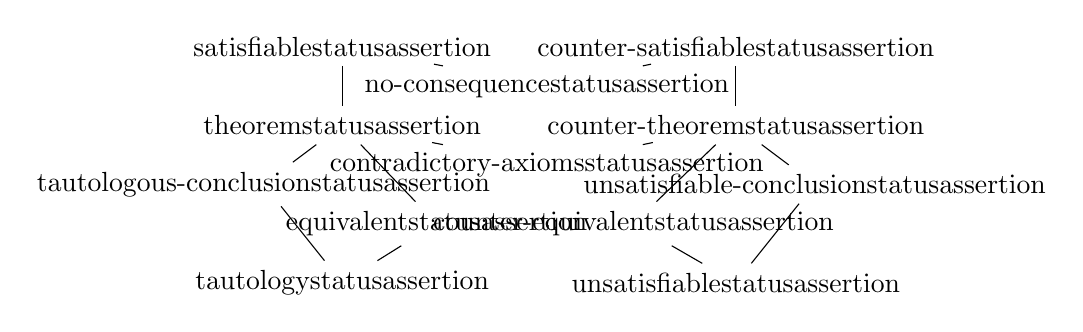
\begin{tikzpicture}
    \node (sat) at (1,4) {\attval{satisfiable}{status}{assertion}};
    \node (csat) at (6,4) {\attval{counter-satisfiable}{status}{assertion}};
    \node (thm) at (1,3) {\attval{theorem}{status}{assertion}};
    \node (cthm) at (6,3) {\attval{counter-theorem}{status}{assertion}};
    \node (tcon) at (0,2.25) {\attval{tautologous-conclusion}{status}{assertion}};
    \node (eqv) at (2.2,1.75) {\attval{equivalent}{status}{assertion}};
    \node (noc) at (3.6,3.5) {\attval{no-consequence}{status}{assertion}};
    \node (cax) at (3.6,2.5) {\attval{contradictory-axioms}{status}{assertion}};
    \node (ceqv) at (4.7,1.75) {\attval{counter-equivalent}{status}{assertion}};
    \node (ucon) at (7,2.25) {\attval{unsatisfiable-conclusion}{status}{assertion}};
    \node (taut) at (1,1) {\attval{tautology}{status}{assertion}};
    \node (usat) at (6,1) {\attval{unsatisfiable}{status}{assertion}};
    \draw (sat) -- (noc);
    \draw (sat) -- (thm);
    \draw (csat) -- (noc);
    \draw (csat) -- (cthm);
    \draw (thm) -- (tcon);
    \draw (thm) -- (cax);
    \draw (cthm) -- (cax);
    \draw (thm) -- (eqv);
    \draw (cthm) -- (ucon);
    \draw (cthm) -- (ceqv);
    \draw (tcon) -- (taut);
    \draw (eqv) -- (taut);
    \draw (ucon) -- (usat);
    \draw (ceqv) -- (usat);
  \end{tikzpicture}
\end{scriptsize}
\end{myfig}
\end{omgroup}

\begin{omgroup}[id=type-assertions]{Type Assertions}

In the last section, we have discussed the \element{type} elements in \element{symbol}
declarations. These were axiomatic (and thus {\indextoo{theory-constitutive}}) in
character, declaring a symbol to be of a certain type, which makes this information
available to type checkers that can check well-typedness (and thus plausibility) of the
represented mathematical objects.

\begin{omtext}
However, not all type information is axiomatic, it can also be deduced from other sources
knowledge. We use the same \element{type} element we have discussed in
\sref{type-axioms} for such \inlinedef{\defii{type}{assertions},
  i.e. non-constitutive statements that inform a type-checker}. In this case, the
\element{type} element can occur at top level, and even outside a \element{theory}
element (in which case they have to specify their home theory in the
\attribute{theory}{type} attribute).
\end{omtext}

{\Mylstref{term-declaration}} contains a type assertion $x+x\colon evens$, which makes the
information that doubling an integer number results in an even number available to the
reasoning process.

\begin{lstlisting}[label=lst:term-declaration,
  caption={A Term declaration in \omdoc.},
  index={type,assertion}]
<type xml:id="double-even.td" system="#POST" 
      theory="adv.int" for="plus" just-by="#double-even">
  <m:math>
    <m:apply><m:plus/>
      <m:ci type="integer">X</m:ci>
      <m:ci type="integer">X</m:ci>
    </m:apply>
  </m:math>
  <m:math>
    <m:csymbol definitionURL="http://cds.omdoc.org/integers/evens"/>
  </m:math>
</type>

<Assertion xml:id="double-even" type="lemma" theory="adv.int">
  <FMP>
    <m:math>
      <m:apply><m:forall/>
        <m:bvar><m:ci xml:id="x13" type="integer">X</m:ci></m:bvar>
        <m:apply><m:in/>
          <m:apply><m:plus/>
            <m:ci definitionURL="x13" type="integer">X</m:ci>
            <m:ci definitionURL="x13" type="integer">X</m:ci>
          </m:apply>
          <m:csymbol definitionURL="http://cds.omdoc.org/nat/evens"/>
        </m:apply>
      </m:apply>
    </m:math>
  </FMP>
</assertion>
\end{lstlisting}
The body of a type assertion contains two mathematical objects, first the type of
the object and the second one is the object that is asserted to have this
type.
\end{omgroup}

\begin{omgroup}[id=alternative]{Alternative Definitions}

  In contrast to what we have said about {\twintoo{conservative}{extension}s} at the end
  of \sref{definitions}, mathematical documents often contain multiple definitions for a
  concept or mathematical object. However, if they do, they also contain a careful
  analysis of equivalence among them. \omdoc allows us to model this by providing the
  \element{alternative} element.  Conceptually, an alternative definition or axiom is
  just a group of assertions that specify the equivalence of logical formulae. Of course,
  alternatives can only be added in a consistent way to a body of mathematical knowledge,
  if it is guaranteed that it is equivalent to the existing ones.  

\begin{definition}[id=alternative.def]
  The \attribute{for}{alternative} on the {\eldef{alternative }} points to the primary
  definition or assertion.  Therefore, \element{alternative} has the attributes
  \attribute{entails}{alternative} and \attribute{entailed-by}{alternative}, that
  specify {\element{assertion}s} that state the necessary entailments. It is an
  {\indextoo{integrity condition}} of \omdoc that any \element{alternative} element
  references at least one \element{definition} or \element{alternative} element that
  entails it and one that it is entailed by (more can be given for convenience). The
  \attribute{entails-thm}{alternative}, and \attribute{entailed-by-thm}{alternative}
  attributes specify the corresponding assertions. This way we can always reconstruct
  equivalence of all definitions for a given symbol. As alternative definitions are not
  theory-constitutive, they can appear outside a \element{theory} element as long as
  they have a \attribute{theory}{alternative} attribute.
\end{definition}
\end{omgroup}

\begin{omgroup}[short=Assertional Statements,id=assertional-statements]{Assertional Statements}

There is another distinction for statements that we will need in the following. Some kinds
of mathematical statements add information about the mathematical objects in question,
whereas other statements do not. For instance, a symbol declaration only declares an
unambiguous name for an object.
\begin{definition}[display=flow,id=assertional.def]
  We will call the following \omdoc elements
  \adefii{assertional}{assertional}{element}: \element{axiom} (it asserts central
  properties about an object), \element{type} (it asserts type properties about an
  object), \element{definition} (this asserts properties of a new object), and of course
  \element{assertion}.
\end{definition}

The following elements are considered non-assertional: \element{symbol} (only a name is
declared for an object), \element{alternative} (here the assertional content is carried
by the \element{assertion} elements referenced in the structure-carrying attributes of
\element{alternative}).  For the elements introduced below we will discuss whether they
are assertional or not in their context. In a nutshell, only statements introduced by the
module {\ADTmodule{spec}} (see \sref{adt}) will be assertional.
\end{omgroup}
\end{module}
\end{omgroup}

\begin{omgroup}[id=examples]{Mathematical Examples in OMDoc}
\begin{module}[id=examples]

In mathematical practice examples play a great role, e.g. in concept formation as
witnesses for definitions or as either supporting evidence, or as counter-examples for
conjectures.  Therefore examples are given status as primary objects in \omdoc.
Conceptually, we model an example $\cE$ as a pair $(\cW,\bA)$, where
$\cW=(\cW_1,\ldots,\cW_n)$ is an $n$-tuple of mathematical objects and $\bA$ is an
assertion. If $\cE$ is an example for a mathematical concept given as an \omdoc symbol
$\bS$, then $\bA$ must be of the form $\bS(\cW_1,\ldots,\cW_n)$.
  
If $\cE$ is an example for a conjecture $\bC$, then we have to consider the situation more
carefully. We assume that $\bC$ is of the form $\cQ\bD$ for some formula $\bD$, where
$\cQ$ is a sequence $\cQ_1W_1,\ldots,\cQ_mW_m$ of $m\geq n=\#\cW$ quantifications of using
quantifiers $\cQ_i$ like $\forall$ or $\exists$.  Now let $\cQ'$ be a sub-sequence of
$m-n$ quantifiers of $\cQ$ and $\bD'$ be $\bD$ only that all the $W_{i_j}$ such that the
$\cQ_{i_j}$ are absent from $\cQ'$ have been replaced by $\cW_j$ for $1\leq j\leq n$.  If
$\cE=(\cW,\bA)$ supports $\bC$, then $\bA=\cQ'\bD'$ and if $\cE$ is a counter-example for
$\bC$, then $\bA=\neg\cQ'\bD'$.
  
\begin{definition}[id=example.def]
  \omdoc specifies this intuition in an {\eldef{example}} element that contains
  mathematical vernacular as a \element[ns-elt=h]{p} elements for the description and
  $n$ mathematical objects (the witnesses). It has the attributes
\begin{description}
\item[\attribute{for}{example}] specifying for which concepts or assertions
    it is an example.  This is a reference to a {\indextoo{whitespace-separated
    list}} of {\indextoo{URI}} references to \element{symbol},
    \element{definition}, or \element{assertion} elements.
\item[\attribute{type}{example}] specifying the aspect, the value is one of
  \attval{for}{type}{example} or \attval{against}{type}{example}
\item[\attribute{assertion}{example}] a reference to the assertion $\bA$
  mentioned above that formally states that the witnesses really form an example for the
  concept of assertion. In many cases even the statement of this is non-trivial
  and may require a proof.
\end{description}
\end{definition}

\element{example} elements are considered
\twinalt{non-assertional}{assertional}{element} in \omdoc, since the assertional part is
carried by the \element{assertion} element referenced in the
\attribute{assertion}{example} attribute.

Note that the list of mathematical objects in an \element{example} element does not
represent multiple examples, but corresponds to the argument list of the symbol, they
exemplify. In the example below, the symbol for monoid is a three-place relation (see the
type declaration in {\mylstref{symbol}}), so we have three witnesses.

\begin{lstlisting}[label=lst:example,mathescape,
  caption={An \omdoc representation of a mathematical example},
  index={example,for,type,assertion}]
<symbol name="strings-over"/>
<definition xml:id="strings.def" for="strings-over">$\ldots$ $A^*$ $\ldots$</definition>
<symbol name="concat"/>
<definition xml:id="concat.def" for="concat">$\ldots$ $::$ $\ldots$</definition>
<symbol name="empty-string"/>
<definition xml:id="empty-string.def" for="empty-string">$\ldots$ $\epsilon$ $\ldots$</definition>
$\ldots$
<assertion xml:id="string.struct.monoid" type="lemma">
  <h:p>$(A^*,::,\epsilon)$ is a monoid.</h:p>
  <FMP>$mon(A^*,::,\epsilon)$</FMP>
</assertion>
$\ldots$
<example xml:id="mon.ex1" for="monoid" type="for"
        assertion="string.struct.monoid">
  <h:p>The set of strings with concatenation is a monoid.</h:p>
  <OMA id="nat-strings">
    <OMS cd="strings" name="strings"/>
    <OMS cd="setname1" name="N"/>
  </OMA>
  <OMS cd="strings" name="concat"/>
  <OMS cd="strings" name="empty-string"/>
</example>

<assertion xml:id="monoid.are.groups" type="false-conjecture">
 <h:p>Monoids are groups.</h:p>
 <FMP>$\allcdot{S,o,e}{mon(S,o,e)\rightarrow\excdot{i}{group(S,o,e,i)}}$</FMP>
</assertion>

<example xml:id="mon.ex2" for="#monoids.are.groups" type="against"
        assertion="strings.isnt.group">
  <h:p>The set of strings with concatenation is not a group.</h:p>
  <OMR href="#nat-strings"/>
  <OMS cd="strings" name="strings"/>
  <OMS cd="strings" name="concat"/>
  <OMS cd="strings" name="empty-string"/>
</example>

<assertion xml:id="strings.isnt.group" type="theorem">
  <h:p>$(A^*,::,\epsilon)$ is a monoid, but there is no inverse function for it.</h:p>
</assertion>
\end{lstlisting}

In {\mylstref{example}} we show an example of the usage of an \element{example} element
in \omdoc: We declare constructor symbols {\snippet{strings-over}}, that takes an
{\indextoo{alphabet}} $A$ as an argument and returns the set $A^*$ of
{\indextoo{strings}s} over $A$, {\snippet{concat}} for {\twintoo{strings}{concatenation}}
(which we will denote by $::$), and {\snippet{empty-string}} for the
{\twintoo{empty}{string}} $\epsilon$.  Then we state that $\cW=(A^*,::,\epsilon)$ is a
monoid in an \element{assertion} with {\snippet{xml:id="string.struct.monoid"}}.  The
\element{example} element with {\snippet{xml:id="mon.ex1"}} in {\mylstref{example}} is
an example for the concept of a monoid, since it encodes the pair $(\cW,\bA)$ where $\bA$
is given by reference to the assertion {\snippet{string.struct.monoid}} in the
\attribute{assertion}{example} attribute.  Example {\snippet{mon.ex2}} uses the pair
$(\cW,\bA')$ as a {\indextoo{counter-example}} to the {\twintoo{false}{conjecture}}
{\snippet{monoids.are.groups}} using the assertion {\snippet{strings.isnt.group}} for
$\bA'$.
\end{module}
\end{omgroup}

\begin{omgroup}[id=inline-statements]{Inline Statements}
\begin{module}[id=inline-statements]
 
Note that the infrastructure for statements introduced so far does its best to mark up the
interplay of formal and informal elements in mathematical documents, and make explicit the
influence of the context and their contribution to it. However, not all statements in
mathematical documents can be adequately captured directly.  Consider for instance the
following situation, which we might find in a typical mathematical textbook.
\begin{sblockquote}
  {\presbf{Theorem 3.12}}: {\presem{In a monoid $M$ the left unit and the right unit
      coincide, we call it the {\presbf{unit}} of $M$.}}
\end{sblockquote}
The overt role of this text fragment is that of a mathematical theorem --- as indicated by
the cue word ``{\presbf{Theorem}}'', therefore we would be tempted represent it as an
\element{omtext} element with the value \attval{theorem}{type}{attribute} for the
\attribute{type}{attribute} attribute. But the relative clause is clearly a
{\indextoo{definition}} (the {\indextoo{definiens}} is even marked in boldface). What we
have here is an aggregated verbalization of two mathematical statements. In a simple case
like this one, we could represent this as follows:

\begin{lstlisting}[mathescape,caption=A Simple-Minded Representation of {\presbf{Theorem 3.12}}]
<assertion type="theorem" style="display=flow">
  <h:p>In a monoid $M$, the left unit and the right unit coincide,</h:p>
</assertion>
<definition for="unit" style="display:flow">
   <h:p>we call it the <term role="definiendum" name="unit">unit</term> of $M$</h:p>
</definition>
\end{lstlisting}

But this representation remains unsatisfactory: the definition is not part of the theorem,
which would really make a difference if the theorem continued after the inline
definition. The real problem is that the inline definition is linguistically a
phrase-level construct, while the \element{omtext} element is a discourse-level
construct. However, as a phrase-level construct, the inline definition cannot really be
taken as stand-alone, but only makes sense in the context it is presented in (which is the
beauty of it; the re-use of context). With the \element[ns-elt=h]{span} element and its
\attribute[ns-elt=h]{verbalizes}{span}, we can do the following:

\begin{lstlisting}[mathescape,caption=An Inline Definition]
<assertion xml:id='unit-unique' type="theorem" >
  <h:p>In a monoid M, the left unit and the right unit coincide,
    <h:span verbalizes="#unit-def">we call it the unit of M</h:span>.</h:p>
</assertion>
<symbol name="unit"/>
<definition xml:id="unit-def" for="unit" just-by='#unit-unique'>
  <h:p>We call the (unique) element of a monoid M that acts as a left 
    and right unit the <term role="definiendum" name="unit">unit</term> of M.</h:p>
</definition>
\end{lstlisting}

thus we would have the phrase-level markup in the proper place, and we would have an
explicit version of the definition which is standalone\footnote{Purists could use the CSS
  attribute \attribute{style}{definition} on the \element{definition} element with
  value {\attvalshort{display:none}{style}} to hides it from the document; it might also
  be placed into another document altogether}, and we would have the explicit relation
that states that the inline definition is an ``abbreviation'' of the standalone
definition.\ednote{we probably also need inline examples and inline assertions, see
  \tracticket{1498}.}
\end{module}
\end{omgroup}

%%%%%%%%%%%%%%%%%%%%%%%%%%%%%%%%%%%%%%%%%%%%%%%%%%%%%%%%%%%%%%%%%%%%%%%%%
% This file is part of the LaTeX sources of the OMDoc 1.6 specification
% Copyright (c) 2015 Michael Kohlhase
% This work is licensed by the Creative Commons Share-Alike license
% see http://creativecommons.org/licenses/by-sa/2.5/ for details
% The source original is at https://github.com/KWARC/OMDoc/doc/spec 
%%%%%%%%%%%%%%%%%%%%%%%%%%%%%%%%%%%%%%%%%%%%%%%%%%%%%%%%%%%%%%%%%%%%%%%%%

\begin{omgroup}[id=proofs,short=Representing Proofs]{Representing Proofs (Module {\PFmodule{spec}})}

\begin{module}[id=proofs-intro]
Proofs form an essential part of mathematics and modern sciences.
\begin{definition}[display=flow,id=proof.conceptual.def]
  Conceptually, a \defi{proof} is a representation of uncontroversial evidence for the
  truth of an {\indextoo{assertion}}.
\end{definition}
  
  The question of what exactly constitutes a proof has been controversially discussed (see
  e.g.~\cite{BarCoh:ecm01}). The clearest (and most radical) definition is given by
  theoretical logic, where a proof is a sequence, or {\indextoo{tree}}, or
  {\atwintoo{directed}{acyclic}{graph}} ({\indextoo{DAG}}) of applications of inference
  rules from a formally defined logical calculus, that meets a certain set of
  well-formedness conditions.  There is a whole zoo of \twinalt{logical
    calculi}{logical}{calculus} that are optimized for various applications. They have in
  common that they are extremely explicit and verbose, and that the proofs even for simple
  theorems can become very large. The advantage of having formal and fully explicit proofs
  is that they can be very easily verified, even by simple computer programs.  We will
  come back to this notion of {\indextoo{proof}} in \sref{proofobjects}.

  In mathematical practice the notion of a proof is more flexible, and more geared for
  consumption by humans: any line of argumentation is considered a proof, if it convinces
  its readers that it could in principle be expanded to a formal proof in the sense given
  above. As the expansion process is extremely tedious, this option is very seldom carried
  out explicitly. Moreover, as proofs are geared towards communication among humans, they
  are given at vastly differing levels of abstraction. From a very informal proof idea for
  the initiated specialist of the field, who can fill in the details herself, down to a
  very detailed account for skeptics or novices which will normally be still well above
  the formal level. Furthermore, proofs will usually be tailored to the specific
  characteristics of the audience, who may be specialists in one part of a proof while
  unfamiliar to the material in others. Typically such proofs have a
  sequence/tree/DAG-like structure, where the leaves are natural language sentences
  interspersed with mathematical formulae (or {\twintoo{mathematical}{vernacular}}).

  Let us consider a proof and its context (\myfigref{pf-example1-math}) as it could be
  found in a typical elementary math. textbook, only that we have numbered the proof steps
  for referencing convenience. {\Myfigref{pf-example1-math}} will be used as a running
  example throughout this chapter.

\begin{myfig}{pf-example1-math}{A Theorem with a Proof.}
\def\kasten{\hfil\null\nobreak\hfill
            \hbox{\vrule\vbox{\hrule width 6 pt\vskip 6pt\hrule}\vrule}
            \par\smallskip}
\fbox{\begin{minipage}{10cm}
    {\presbf Theorem}: {\presem{There are infinitely many prime numbers.}}\\
    {\presbf Proof}: We need to prove that the set $P$ of all prime numbers is not
    finite.
    \begin{center}
      \begin{tabular}{rp{8cm}}
        1. & We proceed by assuming that $P$ is finite and reaching a contradiction.\\
        2. & Let $P$ be finite.\\
        3. & Then $P=\{p_1,\ldots,p_n\}$ for some $p_i$.\\
        4. & Let $q \colon= p_1 \cdots p_n + 1$.\\
        5. & Since for each $p_i \in P$ we have $q > p_i$, we conclude $q \notin P$.\\
        6. & We prove the absurdity by showing that $q$ is prime:\\
        7. & For each $p_i \in P$ we have $q = p_i k + 1$ for some
             natural number $k$, so $p_i$ can not divide $q$;\\
        8. & $q$ must be prime as $P$ is the set of all prime numbers. \\
        9. & Thus we have contradicted our assumption (2) \\
        10. & and proven the assertion.  \kasten
      \end{tabular}
    \end{center}
  \end{minipage}}
\end{myfig}

Since proofs can be marked up on several levels, we will introduce the \omdoc
markup for proofs in stages: We will first concentrate on proofs as structured
texts, marking up the discourse structure in example
{\myfigref{pf-example1-math}}. Then we will concentrate on the justifications of
proof steps, and finally we will discuss the scoping and hierarchical structure of
proofs.

The development of the representational infrastructure in \omdoc has a long history:
From the beginning the format strived to allow structural semantic markup for textbook
proofs as well as accommodate a wide range of formal proof systems without over-committing
to a particular system. However, the proof representation infrastructure from
{\vomdoc{1.1}} turned out not to be expressive enough to represent the proofs in the
{\sc{Helm}} library~\cite{AspPad:hsmw01}. As a consequence, the {\PFmodule{spec}} module
has been redesigned~\cite{AspKohSac:dtdop03} as part of the {\scsys{MoWGLI}}
project~\cite{AspKoht:mimp02}.  The current version of the {\PFmodule{spec}} module is an
adaptation of this proposal to be as compatible as possible with earlier versions of
\omdoc. It has been validated by interpreting it as an implementation of the
{\twintoo{$\overline\lambda\mu\tilde\mu$}{calculus}}~\cite{SacerdotiCoen:enlt05} proof
representation calculus.
\end{module}


\begin{module}[id=proof-structure]
\begin{omgroup}[id=proof-text]{Proof Structure}

In this section, we will concentrate on the structure of proofs apparent in the proof text
and introduce the \omdoc infrastructure needed for marking up this aspect. Even if the
proof in {\myfigref{pf-example1-math}} is very short and simple, we can observe several
characteristics of a typical mathematical proof.  The proof starts with the thesis that is
followed by nine main ``steps'' (numbered from 1 to 10). A very direct representation of
the content of {\myfigref{pf-example1-math}} is given in {\mylstref{primes-omdoc-text}}.

\begin{lstlisting}[label=lst:primes-omdoc-text,mathescape,
  caption={An \omdoc Representation of {\myfigref{pf-example1-math}}.},
  index={symbol,definition}]
<assertion xml:id="a1">
  <h:p>There are infinitely many prime numbers.</h:p>
</assertion>
<proof xml:id="p" for="#a1">
  <omtext xml:id="intro">
    <h:p>We need to prove that the set $P$ of all prime numbers is not finite.</h:p>
  </omtext>
  <derive xml:id="d1">
    <h:p>We proceed by assuming that $P$ is finite and reaching a contradiction.</h:p>
    <method>
      <proof xml:id="p1">
        <hypothesis xml:id="h2"><h:p>Let $P$ be finite.</h:p></hypothesis>
        <derive xml:id="d3">
          <h:p>Then $P=\{p_1,\ldots,p_n\}$ for some $p_i$.</h:p>
          <method><premise xref="#h2"/></method>
        </derive>
        <symbol name="q"/>
        <definition xml:id="d4" for="q" type="informal">
          <CMP>Let $q \stackrel{def}{=} p_1 \cdots p_n + 1$</CMP>
        </definition>
        <derive xml:id="d5">
          <h:p> Since for each $p_i\in P$ we have $q>p_i$, we conclude $q\notin P$.</h:p>
        </derive>  
        <omtext xml:id="c6">
          <h:p>We prove the absurdity by showing that $q$ is prime:</h:p>
        </omtext>  
        <derive xml:id="d7">
          <h:p>For each $p_i \in P$ we have $q = p_i k + 1$ for some
            natural number $k$, so $p_i$ can not divide $q$;</h:p>
          <method><premise xref="#d4"/></method>
        </derive>
        <derive xml:id="d8">
          <h:p>$q$ must be prime as $P$ is the set of all prime numbers.</h:p> 
          <method><premise xref="#d7"/></method>
        </derive>
        <derive xml:id="d9">
          <h:p>Thus we have contradicted our assumption</h:p>
          <method><premise xref="#d5"/><premise xref="#d8"/></method>
        </derive>  
      </proof>
    </method>
  </derive>  
  <derive xml:id="d10" type="conclusion">
    <h:p>This proves the assertion.</h:p>
  </derive>  
</proof>
\end{lstlisting}
\begin{definition}[id=proof.def]
  Proofs are specified by {\eldef{proof}} elements in \omdoc that have the optional
  attributes \attribute[ns-attr=xml]{id}{proof} and \attribute{theory}{proof} and the
  required attribute \attribute{for}{proof}. The \attribute{for}{proof} attribute
  points to the assertion that is justified by this proof (this can be an
  \element{assertion} element or a \element{derive} proof step (see below), thereby
  making it possible to specify expansions of justifications and thus hierarchical
  proofs).
\end{definition}
Note that there can be more than one proof for a given assertion.

\begin{presonly}
\begin{myfig}{qtproof}{The \omdoc Proof Elements}
\begin{scriptsize}
\begin{tabular}{|>{\tt}l|>{\tt}l|>{\tt}p{2.6truecm}|c|>{\tt}p{4.2truecm}|}\hline
{\rm Element}& \multicolumn{2}{l|}{Attributes\hspace*{2.25cm}} & M & Content  \\\hline
             & {\rm Req.}  & {\rm Optional}                    & D &           \\\hline\hline
 proof       &  for         & theory, xml:id, class, style & +   
             & (omtext | derive | hypothesis | symbol | definition)* \\\hline
 proofobject &                 & xml:id, for, class, style, theory & +  & ({\mobjabbr}) \\\hline
 hypothesis  &                 & xml:id, class, style, inductive & -- & CMP*, FMP*  \\\hline
 derive      &                 & xml:id, class, style, type & -- & CMP*, FMP*, method? \\\hline
 method      &                 & xref & -- & ({\mobjabbr} | premise | proof | proofobject)* \\\hline
 premise     & xref            & & -- & EMPTY\\\hline
\end{tabular}
\end{scriptsize}
\end{myfig}
\end{presonly}

\begin{omtext}
The content of a proof consists of a sequence of proof steps, whose {\indextoo{DAG}}
structure is given by \indexalt{cross-referencing}{cross-reference}. These proof steps are
specified in four kinds of \omdoc elements:
\begin{description}
\item[{\element{omtext}}] \omdoc allows this element to allow for intermediate text in
  proofs that does not have to have a logical correspondence to a proof step, but e.g.
  guides the reader through the proof. Examples for this are remarks by the proof author,
  e.g.  an explanation why some other proof method will not work. We can see another
  example in {\mylstref{primes-omdoc-text}} in lines 5-7, where the comment gives a
  preview over the course of the proof.
\item[{\element{derive}}] elements specify normal proof steps that derive a new claim from
  already known ones, from {\indextoo{assertion}s} or {\indextoo{axiom}s} in the current
  theory, or from the {\indextoo{assumption}s} of the assertion that is under
  consideration in the proof.  See for example lines $12ff$ in
  {\mylstref{primes-omdoc-text}} for examples of \element{derive} proof steps that only
  state the local assertion. We will consider the specification of justifications in
  detail in \sref{proofs.justifications} below.  \inlinedef{The {\eldef{derive}} element
    carries an optional \attribute[ns-attr=xml]{id}{derive} attribute for identification
    and an optional \attribute{type}{derive} to single out special cases of proofs
    steps.}
  
  The value \attval{conclusion}{type}{derive} is reserved for the concluding step of a
  proof\footnote{As the argumentative structure of the proof is encoded in the
    justification structure to be detailed in \sref{proofs.justifications}, the
    concluding step of a proof need not be the last child of a proof element.}, i.e. the
  one that derives the assertion made in the corresponding theorem.  
  
  The value \attval{gap}{type}{derive} is used for proof steps that are not justified
  (yet): \inlinedef{we call them \defii{gap}{steps}}. Note that the presence of gap
  steps allows \omdoc to specify {\twintoo{incomplete}{proof}s} as proofs with gap
  steps.
\item[{\element{hypothesis}}] elements allow to specify {\twintoo{local}{assumption}s}
  that allow the hypothetical reasoning discipline needed for instance to specify proof by
  contradiction, by case analysis, or simply to show that $A$ implies $B$, by assuming $A$
  and then deriving $B$ from this local hypothesis. The scope of an hypothesis extends to
  the end of the \element{proof} element containing it. \inlinedef{In
    {\mylstref{primes-omdoc-text}} the classification of step 2 from
    {\myfigref{pf-example1-math}} as the {\eldef{hypothesis}} element {\snippet{h2}}
    forces us to embed it into a \element{derive} element with a \element{proof}
    grandchild, making a structure apparent that was hidden in the original.}
  
  An important special case of hypothesis is the case of
  ``{\twintoo{inductive}{hypothesis}}'', this can be flagged by setting the value of the
  attribute \attribute{inductive}{hypothesis} to \attribute{yes}{inductive}{hypothesis};
  the default value is \attval{no}{inductive}{hypothesis}.

  \setbox0=\hbox{\element{symbol}/\element{definition}}\item[\box0] These elements allow
  to introduce new local symbols that are local to the containing \element{proof} element.
  Their meaning is just as described in \sref{definitions}, only that the role of the
  \element{axiom} element described there is taken by the \element{hypothesis} element. In
  {\mylstref{primes-omdoc-text}} step 4 in the proof is represented by a
  \element{symbol}/\element{definition} pair. Like in the \element{hypothesis} case, the
  scope of this symbol extends to the end of the \element{proof} element containing it.
\end{description}
\end{omtext}

These elements contain an informal (natural language) representation of the proof step in
a multilingual \twinalt{\element{CMP} group}{multilingual}{group} and possibly an
\element{FMP} element that gives a formal representation of the claim made by this proof
step. A \element{derive} element can furthermore contain a \element{method} element
that specifies how the assertion is derived from already-known facts (see the next section
for details). All of the proof step elements have an optional
{\attributeshort[ns-attr=xml]{id}} attribute for identification and the {\css} attributes.

As we have seen above, the content of any proof step is essentially a Gentzen-style sequent; see
{\mylstref{expansion}} for an example. This mixed representation enhances multi-modal
{\twintoo{proof}{presentation}}~\cite{Fiedler:tape97}, and the accumulation of proof
information in one structure. Informal proofs can be formalized~\cite{Baur:susmt99};
formal proofs can be transformed to natural language~\cite{HuangFiedler:pmfp96}. The first
is important, since it will be initially infeasible to totally formalize all
{\twintoo{mathematical}{proofs}} needed for the {\twintoo{correctness}{management}} of the
{\twintoo{knowledge}{base}}.
\end{omgroup}
\end{module}

\begin{module}[id=justifications]
\begin{omgroup}[id=proofs.justifications]{Proof Step Justifications}

\begin{omtext}
  So far we have only concerned ourselves with the linear structure of the proof, we have
  identified the proof steps and classified them by their function in the proof. A central
  property of the \element{derive} elements is that their content (the local claim)
  follows from statements that we consider true. These can be earlier steps in the proof
  or general knowledge. To convince the reader of a proof, the steps are often accompanied
  with \inlinedef{a \defi{justification}}.  This can be given either by a logical
  {\twintoo{inference}{rule}} or {\twintoo{higher-level}{evidence}} for the truth of the
  claim.  The evidence can consist in a {\twintoo{proof}{method}} that can be used to
  prove the assertion, or in a separate subproof, that could be presented if the consumer
  was unconvinced.  Conceptually, both possibilities are equivalent, since the
  {\indextoo{method}} can be used to compute the subproof (\inlinedef{called its
    \defi{expansion}}). Justifications are represented in \omdoc by the
  \element{method} children of \element{derive} elements\footnote{The structural and
    formal justification elements discussed in this section are derived from hierarchical
    data structures developed for semi-automated theorem proving (satisfying the logical
    side). They allow natural language representations at every level (allowing for
    natural representation of mathematical vernacular at multiple levels of abstraction).
    This proof representation (see~\cite{BenzmuellerEtAl:otama97} for a discussion and
    pointers) is a DAG of nodes which represent the proof steps.}  (see
  {\mylstref{derive}} for an example):
\end{omtext}

\begin{definition}[id=method.def]
  The {\eldef{method}} element contains a structural specification of the justification of
  the claim made in the \element{FMP} of a \element{derive} element.
\end{definition}
So the \element{FMP} together with the \element{method} element jointly form the
counterpart to the natural language content of the \element{CMP} group, they are sibling
to: The \element{FMP} formalizes the local claim, and the \element{method} stands for
the justification. In {\mylstref{derive}} the formula in the \element{CMP} element
corresponds to the claim, whereas the part ``By \ldots, we have'' is the justification. In
other words, a \element{method} element specifies a proof method or inference rule with
its arguments that justifies the assertion made in the \element{FMP} elements.  It has
an optional \attribute{xref}{method} attribute whose target is an \omdoc definition of
an {\twintoo{inference}{rule}} or {\twintoo{proof}{method}}.\footnote{At the moment
  \omdoc does not provide markup for such objects, so that they should best be
  represented by \element{symbol}s with \element{definition} where the inference rule
  is explained in the \element{CMP} (see the lower part of {\mylstref{derive}}), and the
  \element{FMP} holds a content representation for the inference rule, e.g.  using the
  content dictionary~\cite{CD:inference-rules}.  A good enhancement is to encapsulate
  system-specific encodings of the inference rules in \element{private} or
  \element{code} elements and have the \attribute{xref}{method} attribute point to
  these.} A method may have {\openmath} objects, {\cmathml} expressions,
\element{legacy}, \element{premise}, \element{proof}, and
\element{proofobject}\footnote{This object is an alternative representation of certain
  proofs, see \sref{proofobjects}.} children.  These act as {\indextoo{parameter}}s to
the method, e.g. for the repeated universal instantiation method in {\mylstref{derive}}
the parameters are the terms to instantiate the bound variables.
  
\begin{definition}[id=premise.def]
  The {\eldef{premise}} elements are used to refer to already established assertions:
  other proof steps or statements --- e.g. ones given as \element{assertion},
  \element{definition}, or \element{axiom} elements --- the method was applied to to
  obtain the local claim of the proof step. The \element{premise} elements are empty and
  carry the required attribute \attribute{xref}{premise}, which contains the URI of the
  assertion.
\end{definition}
Thus the \element{premise} elements specify the {\indextoo{DAG}} structure of the
proof. Note that even if we do not mark up the method in a justification (e.g. if it is
unknown or obvious) it can still make sense to structure the argument in
\element{premise} elements. We have done so in {\mylstref{primes-omdoc-text}} to make
the dependencies of the argumentation explicit.
  
  If a \element{derive} step is a logically (or even mathematically) complex step, an
  expansion into sub-steps can be specified in a \element{proof} or
  \element{proofobject} element embedded into the justifying \element{method} element.
  An embedded proof allows us to specify generic markup for the hierarchic structure of
  proofs. Expansions of nodes justified by method applications are computed, but the
  information about the method itself is not discarded in the process as in tactical
  theorem provers like {\isabelle}~\cite{Paulson:iagtp94} or {\nuprl}~\cite{Constable86}.
  Thus, proof nodes may have justifications at multiple levels of abstraction in an
  hierarchical proof data structure.  Thus the \element{method} elements allow to
  augment the linear structure of the proof by a {\indextoo{tree}}/{\indextoo{DAG}}-like
  secondary structure given by the \element{premise} links. Due to the complex
  hierarchical structure of proofs, we cannot directly utilize the tree-like structure
  provided by {\xml}, but use \indexalt{cross-referencing}{cross-reference}.  The
  \element{derive} step in {\mylstref{derive}} represents an inner node of the proof
  tree/DAG with three children (the elements with identifiers {\snippet{A2}},
  {\snippet{A4}}, and {\snippet{A5}}).

\begin{lstlisting}[label=lst:derive,mathescape,
  caption={A \element{derive} Proof Step},index={derive,method,premise}]
<proof xml:id="proof.2.1.2.proof.D2.1" for="#assertion.2.1.2">
  $\ldots$
  <derive xml:id="D2.1">
    <h:p>By <ref type="cite" xref="#A2"/>, <ref type="cite" xref="#A4"/>, and
       <ref type="cite" xref="#A5"/> we have $z+(a+(-a))=(z+a)+(-a)$.</h:p>
    <FMP>$z+(a+(-a))=(z+a)+(-a)$</FMP>
    <method xref="nk-sorts.omdoc#NK-Sorts.forallistar">
      <OMV name="z"/>
      <OMV name="a"/>
      $-a$
      <premise xref="#A2"/><premise xref="#A4"/><premise xref="#A5"/>
    </method>
  </derive>
  $\ldots$
</proof>
$\ldots$
<theory xml:id="NK-Sorts">
  <metadata>
    <dc:title>Natural Deduction for Sorted Logic</dc:title>
  </metadata>
  
  <symbol name="forallistar">
    <metadata>
      <dc:description>Repeated Universal Instantiation></dc:description>
    </metadata>
  </symbol>
  <definition xml:id="forallistar.def" for="forallistar" type="informal">
    <CMP>Given $n$ parameters, the inference rule $\forall{I}^*$ instantiates 
      the first $n$ universal quantifications in the antecedent with them.</CMP>
  </definition>
  $\ldots$
</theory>
\end{lstlisting}

\begin{omtext}
  In \omdoc the \element{premise} elements must reference proof steps in the current
  proof or statements (\element{assertion} or \element{axiom} elements) in the scope
  of the current theory: \inlinedef{A statement is in \defi{scope} of the \twinalt{current
      theory}{theory}{in scope of}, if its home theory is the current theory or imported
    (directly or indirectly) by the current theory.}
\end{omtext}

Furthermore note that a proof containing a \element{premise} element is not
self-contained evidence for the validity of the \element{assertion} it proves.
Of course it is only evidence for the validity at all (we call such a proof
{\indextoo{grounded}}), if all the statements that are targets of
\element{premise} references have grounded proofs themselves\footnote{For
  \element{assertion} targets this requirement is obvious. Obviously,
  {\element{axiom}s} do not need proofs, but certain forms of definitions need
  well-definedness proofs (see \sref{definitions}). These are included in
  the definition of a grounded proof.} and the reference relation does not contain
cycles. A grounded proof can be made self-contained by inserting the target
statements as \element{derive} elements before the referencing
\element{premise} and embedding at least one \element{proof} into the
\element{derive} as a justification.

Let us now consider another proof example ({\mylstref{expansion}}) to fortify our intuition.

\begin{lstlisting}[label=lst:expansion,mathescape,
  caption={An \omdoc Representation of a Proof by Cases},
  index={proof,derive,method,assumption,conclusion}]
<assertion xml:id="t1" theory="sets">
  <h:p>If $a\in{U}$ or $a\in{V}$, then $a\in{U}\cup{V}$.</h:p>
  <FMP>
    <assumption xml:id="t1_a">$a\in{U}\vee a\in{V}$</assumption>
    <conclusion xml:id="t1_c">$a\in{U}\cup{V}$</conclusion>
  </FMP>
</assertion>
<proof xml:id="t1_p1" for="#t1" theory="sets">
  <omtext xml:id="t1_p1_m1">
    <h:p> We prove the assertion by a case analysis.</h:p>
  </omtext>
  <derive xml:id="t1_p1_l1">
    <h:p>If $a\in{U}$, then $a\in{U}\cup{V}$.</h:p>
    <FMP>
      <assumption xml:id="t1_p1_l1_a">$a\in{U}$</assumption>
      <conclusion xml:id="t1_p1_l1_c">$a\in{U}\cup{V}$</conclusion>
    </FMP>
    <method xref="sk.omdoc#SK.by_definition">$\cup$</method>
  </derive> 
  <derive xml:id="t1_p1_l2">
    <h:p>If $a\in{V}$, then $a\in{U}\cup{V}$.</h:p>
    <FMP>
      <assumption xml:id="t1_p1_l2_a">$a\in{V}$</assumption>
      <conclusion xml:id="t1_p1_l2_c">$a\in{U}\cup{V}$</conclusion>
    </FMP>
    <method xref="sk.omdoc#SK.by_definition">$\cup$</method>
  </derive> 
  <derive xml:id="t1_p1_c">
    <h:p> We have considered both cases, so we have $a\in{U}\cup{V}$.</h:p>
  </derive> 
</proof>
\end{lstlisting}
This \twinalt{proof}{sequent}{proof} is in {\twintoo{sequent}{style}}: The statement of
all local claims is in self-contained {\element{FMP}s} that mark up the statement in
\element{assumption}/\element{conclusion} form, which makes the logical dependencies
explicit. In this example we use inference rules from the calculus ``SK'',Gentzen's
sequent calculus for {\atwintoo{classical}{first-order}{logic}}~\cite{Gentzen:uudlsiii35},
which we assume to be formalized in a theory {\snippet{SK}}.  Note that local assumptions
from the \element{FMP} should not be referenced outside the \element{derive} step they
were made in. In effect, the \element{derive} element serves as a grouping device for
local assumptions.

Note that the same effect as embedding a \element{proof} element into a
\element{derive} step can be obtained by specifying the \element{proof} at top-level
and using the optional \attribute{for}{proof} attribute to refer to the identity of the
enclosing proof step (given by its optional \attribute[ns-attr=xml]{id}{derive}
attribute), we have done this in the proof in {\mylstref{expansion2}}, which expands the
\element{derive} step with identifier {\snippet{t1\_p1\_l1}} in {\mylstref{expansion}}.

\begin{lstlisting}[label=lst:expansion2,mathescape,
  caption={An External Expansion of Step {\snippet{t\_1\_p1\_l1}} in {\mylstref{expansion}}},
  index={proof,derive,method,assumption,conclusion}]
<definition xml:id="union.def" for="union">
  $\psom{\allcdot{P,Q,x}{x\in P\cup Q\Leftrightarrow x\in{P}\vee x\in{Q}}}$
</definition>

<proof xml:id="t1_p1_l1.exp" for="#t1_p1_l1">
  <derive xml:id="t1_p1_l1.d1">
    <FMP>
      <assumption xml:id="t1_p1_l1.d1.a">$a\in{U}$</assumption>
      <conclusion xml:id="t1_p1_l1.d1.c">$a\in{U}$</conclusion>
    </FMP>
    <method xref="sk.omdoc#SK.axiom"/>
  </derive>
  <derive xml:id="t1_p1_l1.l1.d2">
    <FMP>
      <assumption xml:id="t1_p1_l1.d2.a">$a\in{U}$</assumption>
      <conclusion xml:id="t1_p1_l1.d2.c">$a\in{U}\vee a\in{V}$</conclusion>
    </FMP>
    <method xref="sk.omdoc#SK.orR"><premise xref="#t1_p1_l1.d1"/></method>
  </derive>
  <derive xml:id="t1_p1_l1.d3">
    <FMP>
      <assumption xml:id="t1_p1_l1.d3.a">$a\in{U}\vee a\in{V}$</assumption>
      <conclusion xml:id="t1_p1_l1.d3.c">$a\in{U}\cup{V}$</conclusion>
    </FMP>
    <method xref="sk.omdoc#SK.definition-rl">$U$, $V$, $a$
      <premise xref="#unif.def"/>
    </method>
  </derive>
  <derive xml:id="t1_p1_l1.d4">
    <FMP>
      <assumption xml:id="t1_p1_l1.d3.a">$a\in{U}$</assumption>
      <conclusion xml:id="t1_p1_l1.d3.c">$a\in{U}\cup{V}$</conclusion>
    </FMP>
    <method xref="sk.omdoc#SK.cut">
      <premise xref="#t1_p1_l1.d2"/>
      <premise xref="#t1_p1_l1.d3"/>
    </method>
  </derive>
</proof>          
\end{lstlisting}
\end{omgroup}
\end{module}

\begin{module}[id=scoping-proofs]
\begin{omgroup}[id=proofs.scoping]{Scoping and Context in a Proof}

Unlike the {\atwintoo{sequent}{style}{proof}s} we discussed in the last section, many
informal proofs use the \atwintoo{natural}{deduction}{style}~\cite{Gentzen:uudlsiii35},
which allows to reason from local assumptions. We have already seen such hypotheses as
\element{hypothesis} elements in {\mylstref{primes-omdoc-text}}. The main new feature is
that hypotheses can be introduced at some point in the proof, and are discharged later.
As a consequence, they can only be used in certain parts of the proof.  The hypothesis is
inaccessible for inference outside the nearest ancestor \element{proof} element of the
\element{hypothesis}.
  
\begin{omtext}
  Let us now reconsider the proof in {\myfigref{pf-example1-math}}. Some of the steps (2,
  3, 4, 5, 7) leave the thesis unmodified; \inlinedef{these are called
    \defii{forward}{reasoning} or \defiiis{bottom-up}{proof}{step}}, since they are used
  to derive new knowledge from the available one with the aim of reaching the conclusion.
  Some other steps (1, 6) are used to conclude the (current) thesis by opening new
  subproofs, each one characterized with a new local thesis.  \inlinedef{These steps are
    called \defii{backward}{reasoning} or \defiiis{top-down}{proof}{step} steps, since
    they are used to reduce a complex problem (proving the thesis) to several simpler
    problems (the subproofs)}.  In our example, both backward reasoning steps open just
  one new subproof: Step 1 reduces the goal to proving that the finiteness of $P$ implies
  a contradiction; step 5 reduces the goal to proving that $q$ is prime.
\end{omtext}

Step 2 is used to introduce a new hypothesis, whose scope extends from the point where it
is introduced to the end of the current subproof, covering also all the steps inbetween
and in particular all subproofs that are introduced in these. In our example the scope of
the hypothesis that $P$ is finite (step 2 in {\myfigref{pf-example1-math}}) are steps 3 --
8. In an {\twintoo{inductive}{proof}}, for instance, the scope of the
{\twintoo{inductive}{hypothesis}} covers only the proof of the {\twintoo{inductive}{step}}
and not the proof of the base case (independently from the order adopted to present them
to the user).
  
Step 4 is similar, it introduces a new symbol $q$, which is a
{\twintoo{local}{declaration}} that has scope over lines 4 -- 9.  The difference between a
hypothesis and a local declaration is that the latter is used to introduce a variable as a
new element in a given set or type, whereas the former, is used to locally state some
property of the variables in scope. For example, {\emph{``let $n$ be a natural number''}}
is a declaration, while {\emph{``suppose $n$ to be a multiple of 2''}} is a hypothesis.
The introduction of a new hypothesis or local declaration should always be justified by a
proof step that discharges it. In our example the declaration $P$ is discharged in step
10. Note that in contrast to the representation in {\mylstref{primes-omdoc-text}} we have
chosen to view step 6 in {\myfigref{pf-example1-math}} as a top-down proof step rather
than a proof comment.
  
To sum up, every proof step is characterized by a current thesis and a {\emph{\indextoo{context}}},
which is the set of all the local declarations, hypotheses, and local definitions in
scope. Furthermore, a step can either introduce a new hypothesis, definition, or
declaration or can just be a forward or backward reasoning step.  It is a forward
reasoning \element{derive} step if it leaves the current thesis as it is.  It is a
backward reasoning \element{derive} step if it opens new subproofs, each one
characterized by a new thesis and possibly a new context.

\begin{lstlisting}[label=lst:primes-omdoc,mathescape,
  caption={A top-down Representation of the Proof in {\myfigref{pf-example1-math}}.},
  index={symbol,definition}]
<assertion xml:id="a1">
  <h:p>There are infinitely many prime numbers.</h:p>
</assertion>
<proof for="#a1">
  <omtext xml:id="c0">
    <h:p>We need to prove that the set $P$ of all prime numbers is not finite.</h:p>
  </omtext>
  <derive xml:id="d1">
    <h:p> We proceed by assuming that $P$ is finite and reaching a contradiction.</h:p>
    <method xref="nk.omdoc#NK.by-contradiction">
      <proof>
        <hypothesis xml:id="h2"><h:p>Let $P$ be finite.</h:p></hypothesis>
        <derive xml:id="d3"><h:p>Then $P=\{p_1,\ldots,p_n\}$ for some $n$</h:p></derive>
        <symbol name="q"/>
        <definition xml:id="d4" for="q" type="informal">
          <CMP>Let $q \stackrel{def}{=} p_1 \cdots p_n + 1$</CMP>
        </definition>
        <derive xml:id="d5a">
          <h:p>For each $p_i\in P$ we have $q > p_i$</h:p>
          <method xref="#Trivial"><premise xref="#d4"/></method>
        </derive>
        <derive xml:id="d5b">
          <h:p>$q \notin P$</h:p>
          <method xref="#Trivial"><premise xref="#d5"/></method>
        </derive>
        <derive xml:id="d6">
          <h:p>We show absurdity by showing that $q$ is prime</h:p>
          <FMP>$\bot$</FMP>
          <method xref="#Contradiction">
            <premise xref="#d5b"/>
            <proof>
              <derive xml:id="d7a">
                <h:p>
                  For each $p_i \in P$ we have $q = p_i k + 1$ for a given natural number $k$.
                </h:p>
                <method xref="#By_Definition"><premise xref="#d1"/></method>
              </derive>
              <derive xml:id="d7b">
                <h:p>Each $p_i \in P$ does not divide $q$</h:p>
              </derive>
              <derive xml:id="d8">
                <h:p>$q$ is prime</h:p>
                <method xref="#Trivial">
                  <premise xref="#h2"/>
                  <premise xref="#p4"/>
                </method>
              </derive>
            </proof>
          </method>
        </derive>
      </proof>
    </method>
  </derive>
</proof>
\end{lstlisting}

\element{proof} elements are considered to be
\twinalt{non-assertional}{assertional}{element} in \omdoc, since they do not make
assertions about mathematical objects themselves, but only justify such assertions.
The assertional elements inside the proofs are governed by the scoping mechanisms
discussed there, so that using them in a context where assertional elements are
needed, can be forbidden. 
\end{omgroup}
\end{module}

\begin{module}[id=proofobjects]
\begin{omgroup}[id=proofobjects]{Formal Proofs as Mathematical Objects}

\begin{omtext}
  In \omdoc, the notion of fully formal proofs is accommodated by the
  \element{proofobject} element. In logic, \inlinedef{the term \defii{proof}{object}
    is used for term representations of formal proofs via the Curry/Howard/DeBruijn
    Isomorphism} (see e.g.~\cite{Thompson91} for an introduction and
  {\myfigref{proofobject}} for an example).  $\lambda$-terms are among the most succinct
  representations of calculus-level proofs as they only document the inference
  rules. Since they are fully formal, they are very difficult to read and need specialized
  {\atwintoo{proof}{presentation}{system}s} for human consumption. In proof objects
  inference rules are represented as mathematical symbols, in our example in
  {\myfigref{proofobject}} we have assumed a theory {\snippet{PL0ND}} for the calculus of
  {\twintoo{natural}{deduction}} in {\twintoo{propositional}{logic}} which provides the
  necessary symbols (see {\mylstref{plnd}}).
\end{omtext}

\begin{definition}[id=proofobject.def]
  The {\eldef{proofobject}} element contains an optional multilingual group of
  \element{h:p} elements which describes the formal proof as well as a
  {\twintoo{proof}{object}} which can be an {\openmath} object, {\cmathml} expression, or
  \element{legacy} element.
\end{definition}

\begin{myfig}{proofobject}{A Proof Object for the Commutativity of Conjunction}
\setbox0=\hbox{\quad\begin{textnd}
  \ian{\ibn{\ianc{[A\wedge B]}
                 {B}
                 {\wedge{E_r}\hspace{1em}}}
           {\ian{[A\wedge B]}
                {A}
                {\wedge{E_l}}}
           {B\wedge A}
           {\wedge{I}}}
       {A\wedge B\Rightarrow B\wedge A}
       {\Rightarrow\kern-.3em{I}}
\end{textnd}}
\setbox1=\hbox{\begin{minipage}{4.1cm}
\begin{lstlisting}[frame=none,numbers=none,mathescape,label=proofobject,
   index={proofobject,OMBIND,OMS,OMBVAR,OMATTR,OMATP,OMA}]
<proofobject xml:id="ac.p" for="#and-comm">
 <metadata>
  <dc:description>
   Assuming $A\wedge B$ we have $B$ and $A$ 
   from which we can derive $B\wedge A$.
  </dc:description>
 </metadata>
 <OMBIND id="andcom.pf">
  <OMS cd="PL0ND" name="impliesI"/>
  <OMBVAR>
   <OMATTR>
    <OMATP>
     <OMS cd="PL0ND" name="type"/>
     $\psom{A\wedge{B}}$
    </OMATP>
    <OMV name="X"/>
   </OMATTR>
  </OMBVAR>
  <OMA>
   <OMS cd="PL0ND" name="andI"/>
   <OMA>
    <OMA>
     <OMS cd="PL0ND" name="andEr"/>
     <OMV name="X"/>
    </OMA>
    <OMA>
     <OMS cd="PL0ND" name="andEl"/>
     <OMV name="X"/>
    </OMA>
   </OMA>
  </OMA>
 </OMBIND>
</proofobject>
\end{lstlisting}
\end{minipage}}
\setbox2=\hbox{\begin{minipage}{11cm}
  The schema on the left shows the proof as a natural deduction proof tree, the
  \omdoc representation gives the proof object as a $\lambda$ term. This term
  would be written as the following term in traditional (mathematical) notation:
  $\Rightarrow\kern-.3em{I}(\lambda{X:A\wedge{B}}.\wedge\kern-.3em{I}(\wedge{E_r}(X),\wedge{E_l}(X)))$
\end{minipage}}

\begin{tabular}{|cc|}\hline
 \box0 & \box1\\\hline
 \multicolumn{2}{|c|}{\box2}\\\hline
\end{tabular}
\end{myfig}
Note that using \omdoc symbols for inference rules and mathematical objects for proofs
reifies them to the object level and allows us to treat them at par with any other
mathematical objects. We might have the following theory for natural deduction in
propositional logic as a reference target for the second inference rule in
{\myfigref{proofobject}}.

\begin{lstlisting}[label=lst:plnd,mathescape,
  caption={A Theory for Propositional Natural Deduction}]
<theory xml:id="PL0ND">
  <metadata>
    <dc:description>The Natural Deduction Calculus for Propositional Logic</dc:description>
  </metadata>
  $\ldots$
  <symbol name="andI">
    <metadata><dc:subject>Conjunction Introduction</dc:subject></metadata>
    <type system="prop-as-types">$A\to B\to(A\wedge B)$</type>
  </symbol>

  <definition xml:id="andI.def" for="andi">
    <h:p>Conjunction introduction, if we can derive $A$ and $B$, 
      then we can conclude $A\wedge B$.</h:p>
  </definition>
  $\ldots$
</theory>
\end{lstlisting}

In particular, it is possible to use a \element{definition}
element to define a {\atwintoo{derived}{inference}{rule}} by simply specifying the proof
term as a {\indextoo{definiens}}:
\begin{lstlisting}[mathescape]
<symbol name="andcom">
  <metadata><dc:description>Commutativity for $\wedge$</dc:description></metadata>
  <type system="prop-as-types">$(A\wedge B)\to (B\wedge A)$</type>
</symbol>
<definition xml:id="andcom.def" for="#andcom" type="simple">
  <OMR href="#andcom.pf"/>
</definition>
\end{lstlisting}
Like {\element{proof}s}, {\element{proofobject}s} elements are considered to be
\twinalt{non-assertional}{assertional}{element} in \omdoc, since they do not make
assertions about mathematical objects themselves, but only justify such assertions.
\end{omgroup}
\end{module}
\end{omgroup}

%%% Local Variables: 
%%% mode: latex
%%% TeX-master: "main"
%%% End: 

% LocalWords:  pf lst mathescape metacomment qtproof xref foralli NK SK andi
% LocalWords:  orR pd proofobject em OMATP comm cd impliesI openproof andI def
% LocalWords:  andEr andEl proofobjects exp rl unif pt omdoc h:p FMP href andI
% LocalWords:  omtext truecm Gentzen OMV dc FOL OMBIND OMS OMBVAR OMATTR
% LocalWords:  OMA ac ref FoND andcom PL andi OMR Claudio's ns attr ff elt rp
% LocalWords:  MoWGLI forallistar strived Req multi metadata plnd andi andi
% LocalWords:  inbetween andi andI andI andI andI andI


\begin{omgroup}[id=st.strict]{Strict Translations}

  We will now give the a formal\ednote{do we really want to call it ``formal''?} semantics
  of the {\STmodule{spec}} elements in terms of strict \omdoc (see
  \sref{strict}).\ednote{what do we do if there is both FMP and CMPs in an
    axiom?}\ednote{what do we do if there is more than one symbol per
    definition?}\ednote{what do we do for non-simple definitions}

\begin{center}\lstset{frame=none,numbers=none,lineskip=-.7ex,aboveskip=-.5em,belowskip=-1em}
  \begin{tabular}{|p{6cm}|p{6cm}|}\hline
    pragmatic & strict\\\hline
{
\begin{lstlisting}[numbers=none,frame=none,mathescape]
<axiom name="$\llquote{n}$" xml:id="$\llquote{i}$">
  $\llquote{body}$
</axiom>
\end{lstlisting}
}&{
\begin{lstlisting}[numbers=none,frame=none,mathescape]
<object name="$\llquote{n}$" xml:id="$\llquote{i}$">
  $\llquote{body}$
</object>
\end{lstlisting}
}\\\hline{
\begin{lstlisting}[numbers=none,frame=none,mathescape]
<symbol name="$\llquote{n}$">
  <type system="$\llquote{s}$">$\llquote{t}$</type>
</symbol>
<definition type="simple"
            xml:id="$\llquote{i}$" for="$\llquote{n}$">
  $\llquote{body}$
</definition>
\end{lstlisting}
}&{
\begin{lstlisting}[numbers=none,frame=none,mathescape]
<object name="$\llquote{n}$" xml:id="$\llquote{i}$">
  <type system="$\llquote{s}$">$\llquote{t}$</type>
  <definition>$\llquote{body}$</definition>
</object>
\end{lstlisting}
}\\\hline 
\end{tabular}
\end{center}
\end{omgroup}
\end{omgroup}

%%% Local Variables: 
%%% mode: latex
%%% TeX-master: "main"
%%% End: 

% LocalWords:  lang adt lst mathescape en monoide mon qtconst def cd dc cmp om
% LocalWords:  nat eq xref int suc requation exp rec ref qttheory sst dec csat
% LocalWords:  isnt peano ness bvar mtext concat empystrg setname OMR xlink Ai
% LocalWords:  href Luehts MMiSS qaulified mythy Bi CiA CiB escapechar setstar
% LocalWords:  gim mobj CDname elAlg es td adv ci csymbol definitionURL aa cc
% LocalWords:  equiv cdbase openmath ns elt attr cdversion FMP pres af
% LocalWords:  cdrevision cdstatus cdurl cdreviewdate OMBIND OMATTR multi bool
% LocalWords:  metadata arities OMA sgrp forall thm mW inv Req wrt omcd
% LocalWords:  nmueller ple Inline omtext cthm tcon eqv noc cax ceqv ucon usat
% LocalWords:  tgroup omdoc thc
